\documentclass[twocolumn]{article}
\usepackage{graphicx}
\usepackage{url}
\usepackage{amsmath}
\usepackage{amssymb}
\usepackage{amsfonts}
\usepackage{xcolor}
\usepackage{array}
\usepackage{colortbl}
\usepackage{float}
\usepackage{subcaption}
\usepackage{caption}
\usepackage{booktabs}
\usepackage{geometry}
\usepackage{multirow}
\usepackage{hyperref}
\geometry{margin=2.5cm}
\usepackage{authblk}
\usepackage{enumitem}
\usepackage{tikz}
\usetikzlibrary{shapes.geometric,arrows.meta,positioning,fit,backgrounds,calc}
\usepackage{algorithm}
\usepackage{algpseudocode}
\usepackage{amsthm}
\newtheorem{proposition}{Proposition}
\DeclareMathOperator*{\argmax}{arg\,max}
\DeclareMathOperator*{\argmin}{arg\,min}

\title{Stepwise Multi-Objective Finetuning for Triple-Horizon Anomaly Detection:
Horizon-Specific Loss Extension via Pareto-Guided Darwin-G\"{o}del Machine}

\author[1]{Takato Yasuno}
%\affil[1]{Affiliation TBD}
%\affil[ ]{Email: }

\date{}

\begin{document}

\renewcommand{\abstractname}{Abstract}
\renewcommand{\refname}{References}
\renewcommand{\figurename}{Figure}
\renewcommand{\tablename}{Table}

\maketitle

%% ====================================================================
\begin{abstract}
%% ====================================================================

Anomaly detection in pump-facility time series is hindered by severe
class imbalance---fault events occur in fewer than 13\% of observation
windows---and by the dependency of the optimal loss configuration on
the forecast horizon.
Jointly optimizing all hyperparameters (architecture, adapter rank,
loss function, and class weights) causes cross-subspace interference
that degrades Pareto-frontier convergence and wastes the evaluation budget.

We propose \textbf{Stepwise Multi-Objective DGM}, a framework that
applies the Darwin-G\"{o}del Machine (DGM)
self-improvement loop in four sequential phases,
each targeting a distinct parameter subspace while freezing prior discoveries.
Phase~1 selects PatchTST via comparative
LoRA fine-tuning
(AUC~=~0.965 vs.\ 0.529--0.770 for three alternatives).
Phase~2 fixes LoRA rank~=~16 via systematic rank ablation.
Phase~3 optimizes Focal Loss and class weights
over a 4D space via NSGA-II DGM (macro-F1~=~0.776,
500~iterations, 89.6\% Pareto rate).
Phase~4 optimizes PatchTST patch granularity, establishing
patch\_len~=~26, stride~=~16 as the reproducible optimum
(macro-F1~=~0.773).
However, the stepwise approach has a limitation in that it may not fully capture interactions between parameter subspaces,
and fixed hyperparameter values from a prior phase narrow the scope for post-phase search improvement.
Simultaneous optimization of all hyperparameter subspaces could potentially address these limitations, 
but it introduces cross-subspace interference that complicates Pareto-frontier convergence 
and increases the evaluation budget.

Building on these fixed values, we further propose
\textbf{Horizon-Specific 9D DGM}: each forecast horizon
$h \in \{30,60,90\}\,\mathrm{d}$ receives independent Focal Loss
parameters $(\alpha_h, \gamma_h, w_{n,h})$, subject to the
per-horizon normalisation constraint $w_{n,h}+w_{a,h}=W_\mathrm{sum}$.
This design decouples the inherently different loss landscapes of
short-, medium-, and long-range prediction.
Systematic 4D$\to$6D$\to$8D ablation studies confirm that the
phased approach outperforms full joint search by 12.0 points in
macro-F1 (0.776 vs.\ 0.656), validating the structural decomposition.
A transferable finding also emerges: $\alpha_L/r \approx 2.9$ is a stable LoRA scaling law independent
of search dimensionality.
Under this stable LoRA condition, the focal loss and class-weight parameter subspace
can be effectively optimized to improve horizon-specific anomaly detection performance.
This horizon-specific loss design enables tailored 3D optimization under the class-weight-sum constraint 
for each of the triple forecast horizons, enhancing detection accuracy across short-, medium-, and long-range predictions.
\end{abstract}

\noindent
\textbf{Keywords:} Anomaly Detection, PatchTST, Darwin-G\"{o}del Machine,
Multi-Objective Pareto Optimization, NSGA-II, Horizon-Specific Focal Loss.

%% ====================================================================
\section{Introduction}
\label{sec:intro}
%% ====================================================================

\subsection{Background and Motivation}

Infrastructure facilities such as pump equipment require continuous
condition monitoring to prevent unexpected failures~\cite{mlit2023bridge}.
Time-series anomaly detection using transformer architectures has
shown promise, yet the class imbalance between normal and anomalous
states---fault events occur in fewer than 13\% of time windows---
remains a fundamental challenge.

PatchTST~\cite{nie2023patchtst} is a patch-based time-series
transformer that treats temporal patches as input tokens,
analogous to ViT~\cite{dosovitskiy2020vit} in vision.
When fine-tuned with LoRA~\cite{hu2022lora} for anomaly classification,
it achieves competitive detection metrics on pump-facility sensor data.
Focal Loss~\cite{lin2017focal} addresses class imbalance by
down-weighting easy examples via focusing factor $\gamma$,
combined with per-sample class weights.
However, the combined hyperparameter space---model architecture,
adapter rank, and loss function---spans many interdependent dimensions
and resists analytical treatment.

\subsection{Darwin-G\"{o}del Machine for Horizon-Specific Improvement}

The Darwin-G\"{o}del Machine (DGM)~\cite{liu2025dgm} operationalises
open-ended self-improvement: LLM-based coding agents propose
parameter modifications, a fitness function evaluates each proposal,
and accepted solutions seed future generations.
In a preceding study~\cite{yasuno2026dgm}, we applied DGM to
10-class damage-cause encoding, demonstrating that NSGA-II
multi-objective DGM yields 11 Pareto-optimal solutions
(macro-accuracy 0.840--0.958) from a single 50-iteration run.
This paper extends DGM with a \emph{phased strategy}:
each run targets one parameter subspace at a time.
The stepwise approach mitigates cross-subspace interference by isolating the optimization 
of each hyperparameter subspace under prior phase discoveries.
Furthermore, this phased strategy is naturally extended to simultaneous hyperparameter search:
a 4D, 6D, 8D gradual progression for effective range exploration in each horizon-consistent subspace.
However, simultaneous search across multiple subspaces has limitations in improving horizon-specific accuracy
due to the increased complexity of horizon feature representation.
This paper proposes a stepwise, horizon-specific optimization framework for hyperparameter search, 
mitigating cross-subspace interference and enhancing triple-horizon improvement.

\subsection{Contributions}

\begin{enumerate}[leftmargin=*,topsep=2pt,itemsep=1pt]
  \item \textbf{Stepwise Multi-Objective DGM (4 Phases):}
        Principled decomposition of the PatchTST hyperparameter
        space; each phase freezes prior discoveries to prevent
        cross-subspace interference.
        Model Selection (Phase~1): Comparative LoRA finetuning of AnomalyBERT, PatchTST,
        Chronos~\cite{ansari2024chronos}, and TimesFM~\cite{das2024timesfm};
        PatchTST selected for AUC~=~0.965(60d).
        LoRA Ablation (Phase~2): Systematic study of rank~=~16.
        4D Focal Loss DGM (Phase~3): Best: $\alpha$=0.866, $\gamma$=1.156,
        $w_n$=1.851, $w_a$=4.035.
        2D Architecture DGM (Phase~4): optimum at $L_p{=}26$, $s{=}16$.
  \item \textbf{Structured Joint optimization:}
        Systematic 4D$\to$6D$\to$8D progression (F1: 0.614$\to$0.642$\to$0.656);
        three empirical findings---
        LoRA $\alpha/r{\approx}2.9$ scaling law,
        near-balanced class weights optimal under Focal Loss,
        and weak cross-component interactions---
        confirm the stepwise decomposition as the correct structural prior.
  \item \textbf{Horizon-Specific 9D DGM:}
        Extends the joint optimization framework to assign
        independent Focal Loss parameters
        $(\alpha_h, \gamma_h, w_{n,h})$ per forecast horizon
        $h\in\{30,60,90\}\,\mathrm{d}$, subject to
        $w_{n,h}+w_{a,h}=5.88$.
        Extended to 3{,}000 iterations, the search
        attains a best macro-F1 of 0.769 (30d F1~=~0.789),
        surpassing the 8D joint baseline by +11.3 points.        
\end{enumerate}

\subsection{Phased DGM Framework and Horizon-Specific Extension}

Figure~\ref{fig:phased_overview} illustrates the four-phase
intelligence harness framework.
Each phase targets a distinct parameter subspace,
with outputs feeding forward to constrain subsequent phases.
The central AI-driven DGM loop orchestrates multi-objective
optimization across time-series model selection, LoRA ablation,
loss function tuning, and architecture constraint enforcement.
In the stepwise multi-objective DGM framework, each phase incrementally refines 
a horizon consistent subset of hyperparameters: architecture (patch length, stride) 
and parameter efficient fine-tuning (LoRA $r, \alpha$). 
However, the loss function parameters (focal loss $\alpha, \gamma$ and class weights $w_n, w_a$) 
are optimized horizon-specifically to account for their distinct effects on the three forecast horizons' performance.
Therefore, this paper extends to a horizon-specific 9D ($=$3D$\times$3H) DGM framework that separates the 
loss-function hyperparameters across different forecast horizons under the constraint on the sum of class weights.

\begin{figure}
\centering
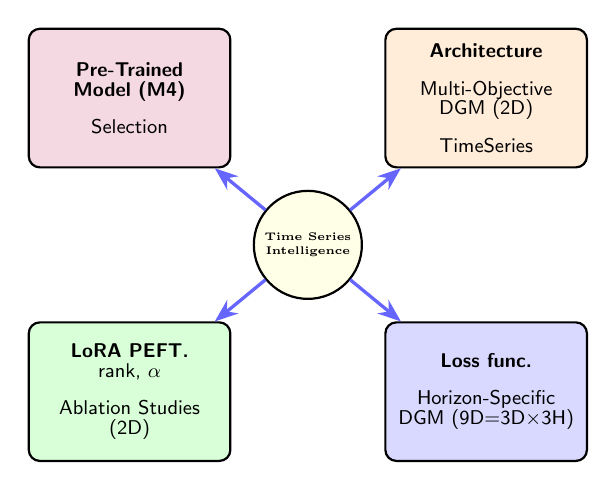
\begin{tikzpicture}[
  scale=0.8, transform shape,
  node distance=0.3cm,
  box/.style={draw, thick, rounded corners=4pt,
              minimum width=3.2cm, minimum height=2.2cm,
              font=\small\sffamily, align=center},
  arr/.style={-Stealth, very thick, blue!60},
  label/.style={font=\scriptsize\bfseries}
]
% Central circle
\node[draw, circle, thick, minimum size=1.6cm,
      fill=yellow!10, font=\tiny\bfseries, align=center] (center)
      {Time Series\\ Intelligence};

% Four quadrants
\node[box, fill=purple!15, above left=0.6cm and 0.6cm of center] (phase1)
      {\textbf{Pre-Trained}\\[-2pt]\textbf{Model (M4)}\\[6pt]Selection};
\node[box, fill=green!15, below left=0.6cm and 0.6cm of center] (phase2)
      {\textbf{LoRA PEFT.}\\[-2pt]rank, $\alpha$\\[6pt]Ablation Studies\\[-2pt](2D)};
\node[box, fill=blue!15, below right=0.6cm and 0.6cm of center] (phase3)
      {\textbf{Loss func.}\\[6pt]Horizon-Specific\\[-2pt]DGM (9D$=$3D$\times$3H)};
\node[box, fill=orange!15, above right=0.6cm and 0.6cm of center] (phase4)
      {\textbf{Architecture}\\[6pt]Multi-Objective\\[-2pt]DGM (2D)\\[6pt]TimeSeries};

% Arrows from center to phases
\draw[arr] (center) -- (phase1);
\draw[arr] (center) -- (phase2);
\draw[arr] (center) -- (phase3);
\draw[arr] (center) -- (phase4);

\end{tikzpicture}
\caption{Phased DGM framework for PatchTST optimization.
The central AI orchestrates four specialised phases:
(1)~Model Selection from pre-trained M4 candidates,
(2)~LoRA PEFT Ablation Studies and Multi-Objective DGM (2D: rank, scaling),
(3)~Horizon-Specific Class Weighted Focal Loss DGM (9D$=$3D$\times$3H, constraint on the sum of weights),
(4)~Architecture DGM (2D: patch\_len, stride).
Each phase freezes prior discoveries to prevent cross-subspace interference.}
\label{fig:phased_overview}
\end{figure}

%% ====================================================================
\section{Related Work}
\label{sec:related}
%% ====================================================================

\subsection{Time-Series Transformer Architectures for Anomaly Detection}

PatchTST~\cite{nie2023patchtst} achieves strong long-term forecasting
performance by segmenting the input into patch tokens, analogous to
ViT~\cite{dosovitskiy2020vit} in computer vision.
The patch-based tokenization reduces sequence length and improves
local temporal coherence.
The original Transformer~\cite{vaswani2017attention} established the
self-attention mechanism underlying all modern sequence models;
Informer~\cite{zhou2021informer} reduced its quadratic complexity to
$O(N\log N)$ via ProbSparse attention, enabling long-range forecasting.
AnomalyBERT~\cite{jeong2023anomalybert} applies BERT-style
self-supervised pre-training to time-series anomaly detection.
Foundation models Chronos~\cite{ansari2024chronos} (T5-based)
and TimesFM~\cite{das2024timesfm} (decoder-only) offer zero-shot
generalization but require substantially more parameters for
effective fine-tuning on small domain-specific datasets.
Our Phase~1 comparison demonstrates that PatchTST achieves superior
AUC/FPR balance on pump-facility data with only 49K trainable
parameters, at a fraction of the cost of foundation models.

Transformer-based anomaly detectors have advanced the state of the art
on multivariate sensor data.
Anomaly Transformer~\cite{xu2022anomaly} introduces an
association-discrepancy criterion that measures the divergence between
prior association and series association to identify anomalies without
requiring labels.
OmniAnomaly~\cite{su2019omni} uses stochastic recurrent networks
(GRU-VAE) with planar normalizing flows to model the distribution of
normal multivariate time series.
USAD~\cite{audibert2020usad} employs adversarially trained
autoencoders to amplify reconstruction errors for anomalous inputs.
TranAD~\cite{tuli2022tranad} combines a Transformer encoder with
adversarial training and a focus score mechanism tailored for
multi-entity industrial IoT data.
In contrast to these unsupervised reconstruction-based methods,
our approach operates in a supervised binary-classification setting
with labelled inspection records, enabling direct optimization of
precision, recall, and FPR per forecast horizon.

\subsection{Focal Loss, Class-Imbalance Learning and PEFT}

Focal Loss~\cite{lin2017focal} was originally proposed for dense
object detection, down-weighting easy examples via the focusing
factor $\gamma$.
For binary anomaly detection, class imbalance is severe: fault
events may occur in fewer than 10\% of time windows.
Standard cross-entropy biases models toward the majority class;
Focal Loss mitigates this but requires careful joint tuning of
$\alpha$, $\gamma$, and per-class weights.
SMOTE~\cite{chawla2002smote} addresses imbalance by synthesizing
minority-class examples through feature-space interpolation,
but cannot be straightforwardly applied to sequential sensor data
without disrupting temporal structure.
Cost-sensitive learning~\cite{he2009adasyn} adjusts the
misclassification penalty asymmetrically, a strategy that overlaps
with per-class weight tuning.
The present paper automates this joint tuning via multi-objective
DGM, removing the need for manual heuristic selection.

LoRA~\cite{hu2022lora} inserts low-rank adapter matrices into frozen
Transformer weight matrices, enabling efficient fine-tuning with
approximately 1--10\% of total parameters.
The rank $r$ and scaling factor $\alpha_L$ jointly control the
adapter capacity; the ratio $\alpha_L/r$ governs the effective
learning rate of the adapter.
Phase~2 ablation over $r \in \{8,12,16,20,32,64\}$ confirms
rank~=~16 as the Pareto-optimal operating point for PatchTST
on the pump-facility Golden Testset, consistent with findings
from NAS~\cite{elsken2019nas} that moderate-capacity adapters
outperform both under- and over-parameterized configurations.

\subsection{Multi-Objective Evolutionary Computation and Hyperparameter Optimization}

NSGA-II~\cite{deb2002nsga2} remains the standard baseline for
multi-objective evolutionary optimization due to its efficient
non-dominated sorting and crowding-distance diversity mechanism.
NSGA-III~\cite{deb2014nsga3} extends NSGA-II to many-objective
problems ($\geq 4$ objectives) via reference-point-based selection,
and is better suited to objectives exceeding eight dimensions.
SPEA2~\cite{zitzler2001spea2} maintains an external archive of
non-dominated solutions and uses a fitness assignment strategy
based on strength values and raw fitness.
The hypervolume indicator~\cite{zitzler2003hypervolume} provides
a unary quality measure of a Pareto approximation set;
its computation is exponential in the number of objectives, but
feasible for the 15-objective vector used in this work.
Our framework wraps NSGA-II via Optuna~\cite{akiba2019optuna}
with a tell/ask interface that enables the LLM validator to
intercept and micro-correct proposals before evaluation.

Hyperband~\cite{li2017hyperband} achieves near-optimal simple
regret by adaptively allocating the training budget among
configurations using successive halving.
BOHB~\cite{falkner2018bohb} combines Hyperband with
Bayesian optimization (TPE~\cite{bergstra2011algorithms}) to
exploit model-based guidance while retaining Hyperband's
early-stopping efficiency.
Neural Architecture Search (NAS)~\cite{elsken2019nas} automates
model design via evolutionary, gradient-based, or
reinforcement-learning strategies; our Phase~4 maps to a
small 2D grid-constrained NAS over patch granularity.
FunSearch~\cite{romera2023funsearch} uses LLMs to evolve
mathematical programs that improve on human-designed baselines,
demonstrating the generality of LLM-guided search beyond
software engineering tasks.
The DGM framework~\cite{liu2025dgm} and our extension differ
from AutoML pipelines in that the LLM validates proposals
with domain-specific anomaly detection context rather than
treating the search as a black-box function evaluation.

\subsection{Self-Improvement Agents and Darwin-G\"{o}del Machine}

\textbf{LLM-based self-improvement.}
Early work on self-improving agents focused on verbal reinforcement:
Reflexion~\cite{shinn2024reflexion} stores episodic feedback in a
linguistic memory and revisits failed trajectories without weight updates;
ReAct~\cite{yao2023react} interleaves reasoning traces with environment
actions, enabling chain-of-thought grounding.
ExpEL~\cite{zhao2024expel} extends this with experiential replay,
accumulating task-specific insight across episodes.
PromptBreeder~\cite{fernando2023promptbreeder} automates meta-prompt
evolution via self-referential mutation, showing that the instruction
itself can be the optimisation target.

\textbf{Open-ended and automated discovery.}
OPRO~\cite{yang2024opro} frames optimisation as LLM meta-prompting,
solving combinatorial tasks by iteratively refining solution
candidates in context.
ADAS~\cite{hu2024adas} searches the space of agentic system designs,
evolving agent architectures rather than fixed hyperparameters.
AI Scientist~\cite{lu2024ai} automates end-to-end research: idea
generation, experiment execution, result analysis, and paper writing.
Quiet-STaR~\cite{zelikman2024quiet} teaches models to produce internal
rationales before committing to outputs, improving sample efficiency
in few-shot settings.
LLM-guided EMO~\cite{nie2025llm} integrates LLM proposals directly
into evolutionary multi-objective optimisation loops, reducing
function evaluations needed to approximate the Pareto front.
Agentless~\cite{chen2024agentless} demonstrates that structured,
plan-then-execute agents can match or exceed complex agent frameworks
on software engineering benchmarks at lower cost.

\textbf{Darwin-G\"{o}del Machine.}
DGM~\cite{liu2025dgm} operationalizes the G\"{o}del
Machine~\cite{schmidhuber2003goedel} framework with LLM-based
coding agents validated on SWE-bench.
Eureka~\cite{ma2024eureka} demonstrates LLM-designed reward
functions that surpass human experts on robotic control.
In a preceding study~\cite{yasuno2026dgm}, we applied DGM to
10-class damage-cause encoding, demonstrating that NSGA-II
multi-objective DGM yields 11 Pareto-optimal solutions
(macro-accuracy 0.840--0.958) from a single 50-iteration run.
The present paper scales DGM to a 15-objective, multi-phase
hyperparameter search with a horizon-specific parameter design
that is novel to the anomaly detection literature.

%% ====================================================================
\section{Problem Formulation}
\label{sec:problem}
%% ====================================================================

\subsection{PatchTST Anomaly Classifier}

Given a univariate time series $\mathbf{x} \in \mathbb{R}^{T}$
($T{=}90$ days), PatchTST divides it into $N_p$ patches of length
$L_p$ with stride $s$:
\begin{equation}
  N_p = \left\lfloor\frac{T - L_p}{s}\right\rfloor + 1.
  \label{eq:npatch}
\end{equation}
The patches are linearly projected and passed through a Transformer
encoder~\cite{vaswani2017attention} to produce classification logits
$\hat{\mathbf{y}} \in \mathbb{R}^3$
for three binary anomaly horizons $h\in\mathcal{H}=\{30,60,90\}\,\mathrm{d}$.
LoRA adapters (rank $r$, scaling $\alpha_\text{L}$) are inserted
into the attention projection layers; all backbone weights are frozen.

\subsection{Horizon-Specific Weighted Focal Loss}

For each horizon $h$ and training sample $i$, the per-instance
weighted Focal Loss is:
\begin{equation}
  \ell_{i,h}(\boldsymbol{\theta}_h)
  = c_{i,h}\cdot
    \mathrm{FL}\!\left(\hat{y}_{i,h},\, y_{i,h};\, \alpha_h, \gamma_h\right)
  \label{eq:instance_loss}
\end{equation}
where the Focal Loss kernel~\cite{lin2017focal} is
\begin{equation}
  \mathrm{FL}(p_t;\alpha_h,\gamma_h)
  = -\alpha_{y,h}(1-p_t)^{\gamma_h}\log p_t,
  \label{eq:focal_kernel}
\end{equation}
\begin{equation}
  \alpha_{y,h} = \begin{cases}
    \alpha_h   & y{=}1,\\
    1-\alpha_h & y{=}0,
  \end{cases}
  \label{eq:fl_kernel}
\end{equation}
$p_t = \sigma(\hat{y}_{i,h})\cdot y_{i,h}
       + (1-\sigma(\hat{y}_{i,h}))\cdot(1-y_{i,h})$
is the model probability for the ground-truth class,
and the per-sample class weight is
\begin{equation}
  c_{i,h} = w_{a,h}\,y_{i,h} + w_{n,h}(1-y_{i,h}).
  \label{eq:classweight}
\end{equation}
The horizon-average training loss over $N$ samples is:
\begin{equation}
  \mathcal{L}(\boldsymbol{\Theta}_H)
  = \frac{1}{|\mathcal{H}|}\sum_{h\in\mathcal{H}}
    \frac{1}{N}\sum_{i=1}^{N}\ell_{i,h}(\boldsymbol{\theta}_h)
  \label{eq:total_loss}
\end{equation}
where $\boldsymbol{\Theta}_H = \{\boldsymbol{\theta}_h\}_{h\in\mathcal{H}}$
collects all horizon-specific parameters.

\textbf{Threshold optimization.}
For each horizon $h$, the decision threshold is calibrated on the
validation set by maximizing $F1$:
\begin{equation}
  \tau_h^* = \argmax_{\tau\in[0.1,\,0.9]}
    F1\!\left(\{(\hat{y}_{i,h},y_{i,h})\}_{\text{val}};\,\tau\right).
  \label{eq:threshold}
\end{equation}
The threshold grid spacing is $0.01$, giving 81 candidate values.

\subsection{Multi-Objective Pareto Formulation}

\textbf{Objective vector.}
Each fine-tuning run with parameters $\boldsymbol{\theta}$
produces a 15-dimensional evaluation vector:
\begin{equation}
  \mathbf{f}(\boldsymbol{\theta}) =
  \bigl(
    \underbrace{\mathrm{AUC}_h, P_h, R_h, F1_h}_{\text{maximise},\;\times 3},\;
    \underbrace{-\mathrm{FPR}_h}_{\text{maximise (negated)},\;\times 3}
  \bigr)
  \in \mathbb{R}^{15}.
  \label{eq:objectives}
\end{equation}
FPR objectives are negated internally so that all 15 dimensions are
maximised, enabling standard NSGA-II dominance comparison.

\textbf{Pareto dominance.}
Solution $\boldsymbol{\theta}$ \emph{dominates} $\boldsymbol{\theta}'$,
written $\boldsymbol{\theta}\prec\boldsymbol{\theta}'$, if and only if
\begin{equation}
  f_j(\boldsymbol{\theta}) \geq f_j(\boldsymbol{\theta}')
  \;\forall j\in[15]
  \quad\text{and}\quad
  \exists\, j:\; f_j(\boldsymbol{\theta}) > f_j(\boldsymbol{\theta}').
  \label{eq:dominance}
\end{equation}
The \emph{Pareto front} is
$\mathcal{P}^* = \{\boldsymbol{\theta}\in\mathcal{H}
  \mid \nexists\,\boldsymbol{\theta}'\in\mathcal{H}:
  \boldsymbol{\theta}'\prec\boldsymbol{\theta}\}$.

\subsection{Phased Search Space Definitions}

\textbf{Phase~3 (4D Focal Loss).}
Architecture ($L_p{=}30$, $s{=}30$) and LoRA ($r{=}16$,
$\alpha_\text{L}{=}32$) are fixed; the search space is:
\begin{equation*}
  \boldsymbol{\theta}_3 =
  (\alpha_\text{FL},\gamma,w_n,w_a),\quad
  \alpha_\text{FL} \in [0.1,0.9],\;
  \gamma \in [0.5,5.0],\;
\end{equation*}
\begin{equation*}
  w_n \in [0.1,5.0],\;
  w_a \in [0.5,10.0].
\end{equation*}

\textbf{Phase~4 (2D Architecture).}
Focal Loss is fixed at Phase~3 optimal values; the search space is:
\begin{equation*}
  \boldsymbol{\theta}_4 = (L_p,s),\quad
  L_p \in [20,32],\quad s \in [10,20].
\end{equation*}

\textbf{Horizon-specific 9D (v0.2.1H).}
Architecture and LoRA are fixed; the search space is:
\begin{equation}
  \boldsymbol{\Theta}_H = \{(\alpha_h,\gamma_h,w_{n,h})\}_{h\in\mathcal{H}},
\end{equation}
\begin{equation}
  \quad
  \alpha_h\in[0.5,0.9],\;
  \gamma_h\in[0.6,2.0],\;
  w_{n,h}\in[0.3,5.5],
  \label{eq:9d_space}
\end{equation}
with the per-horizon normalisation constraint
$w_{n,h}+w_{a,h}=W_\mathrm{sum}=5.88$ for all $h$.
The anomaly-class weight is derived as
$w_{a,h}=W_\mathrm{sum}-w_{n,h}$, reducing the free variables to
three per horizon (nine total).

%% ====================================================================
\section{Methodology}
\label{sec:method}
%% ====================================================================

\subsection{Stepwise optimization Overview}

Figure~\ref{fig:phase_flow} illustrates the four-phase strategy.
Each phase produces fixed optimal values passed forward as frozen
hyperparameters to subsequent phases.

\begin{figure}
\centering
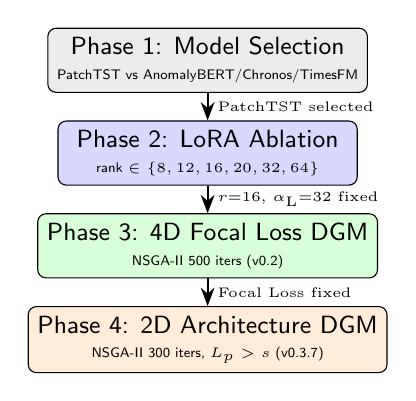
\begin{tikzpicture}[
  node distance=0.35cm,
  ph/.style={draw, rounded corners=3pt,
             minimum width=3.8cm, minimum height=0.7cm,
             font=\small\sffamily, align=center},
  arr/.style={-Stealth, thick}
]
\node[ph, fill=gray!15]   (p1) {Phase~1: Model Selection\\[-2pt]{\tiny PatchTST vs AnomalyBERT/Chronos/TimesFM}};
\node[ph, fill=blue!15,  below=of p1] (p2) {Phase~2: LoRA Ablation\\[-2pt]{\tiny rank $\in\{8,12,16,20,32,64\}$}};
\node[ph, fill=green!15, below=of p2] (p3) {Phase~3: 4D Focal Loss DGM\\[-2pt]{\tiny NSGA-II 500 iters (v0.2)}};
\node[ph, fill=orange!15,below=of p3] (p4) {Phase~4: 2D Architecture DGM\\[-2pt]{\tiny NSGA-II 300 iters, $L_p>s$ (v0.3.7)}};
\draw[arr] (p1) -- (p2) node[midway,right,font=\tiny]{PatchTST selected};
\draw[arr] (p2) -- (p3) node[midway,right,font=\tiny]{$r{=}16$, $\alpha_\text{L}{=}32$ fixed};
\draw[arr] (p3) -- (p4) node[midway,right,font=\tiny]{Focal Loss fixed};
\end{tikzpicture}
\caption{Four-phase stepwise optimization. Each phase freezes prior
discoveries and passes optimal values to the next phase.}
\label{fig:phase_flow}
\end{figure}

\subsection{Phase~1: Model Selection}
\label{subsec:phase1}

Four architectures were LoRA fine-tuned (rank~16) on pump and HVAC
facility data and compared on 60d AUC (Table~\ref{tab:model_select}).
PatchTST (AUC~=~0.965, F1~=~0.815, FPR~=~0.011) outperforms
AnomalyBERT by~+0.195 AUC and foundation models Chronos and TimesFM
by large margins, using only 49K trainable parameters.
PatchTST is selected for all subsequent phases.

\begin{table}
\centering
\caption{Model selection (60d metrics, LoRA fine-tuned).}
\label{tab:model_select}
\small
\renewcommand{\arraystretch}{1.05}
\setlength{\tabcolsep}{4pt}
\begin{tabular}{lrrrr}
\toprule
\textbf{Model} & \textbf{Params} & \textbf{AUC} & \textbf{F1} & \textbf{FPR} \\
\midrule
\rowcolor{green!10}
\textbf{PatchTST} & \textbf{49K} & \textbf{0.965} & \textbf{0.815} & \textbf{0.011} \\
AnomalyBERT~\cite{jeong2023anomalybert} & 115K & 0.770 & 0.378 & 0.139 \\
Chronos~\cite{ansari2024chronos} & 1.18M & 0.565 & --- & --- \\
TimesFM~\cite{das2024timesfm} & 2.46M & 0.529 & --- & --- \\
\bottomrule
\end{tabular}
\end{table}

\subsection{Phase~2: LoRA Rank Ablation}
\label{subsec:phase2}

We ablated rank $r \in \{8, 12, 16, 20, 32, 64\}$ with
$\alpha_\text{L} = 2r$ on the Golden Testset
(Table~\ref{tab:lora_ablation}).
Rank~8 shows degraded average AUC (0.745) due to insufficient
adapter capacity.
Ranks 20--64 add parameters without improving AUC over rank~16,
indicating overfitting of the adapter.
Rank~16 ($\alpha_\text{L}$~=~32, 7.49\% trainable parameters)
is the Pareto-optimal operating point.

\begin{table}
\centering
\caption{LoRA ablation: average AUC, F1, FPR across 30/60/90d.}
\label{tab:lora_ablation}
\small
\renewcommand{\arraystretch}{1.05}
\setlength{\tabcolsep}{4pt}
\begin{tabular}{rrrrr}
\toprule
$r$ & \textbf{\%} & \textbf{AUC} & \textbf{F1} & \textbf{FPR} \\
\midrule
8  & 3.89  & 0.745 & 0.377 & 0.453 \\
12 & 5.73 & 0.897 & 0.609 & 0.090 \\
\rowcolor{green!10}
\textbf{16} & \textbf{7.49} & \textbf{0.947} & \textbf{0.741} & \textbf{0.022} \\
20 & 9.19  & 0.909 & 0.631 & 0.102 \\
32 & 13.94 & 0.902 & 0.627 & 0.082 \\
64 & 24.47 & 0.911 & 0.631 & 0.105 \\
\bottomrule
\end{tabular}
\end{table}

\subsection{Phase~3: 4D Focal Loss DGM}
\label{subsec:phase3}

With LoRA fixed at Phase~2 values, we applied the DGM loop to
$\boldsymbol{\theta}_3$ for 500~iterations (v0.2).
The DGM loop adopts the five-module design of~\cite{yasuno2026dgm}:

\begin{enumerate}[leftmargin=*,topsep=2pt,itemsep=1pt]
  \item \textbf{Archive:} JSONL-backed store of all evaluated
        $(\boldsymbol{\theta}, \mathbf{f})$ pairs.
  \item \textbf{NSGA-II Sampler:} Optuna NSGA-II (population~=~20)
        proposes $\boldsymbol{\theta}$ exploring the 15-objective
        Pareto front.
  \item \textbf{LLM Validator (Codestral 22B):} Validates the NSGA-II
        proposal; applies micro-corrections if counter-productive;
        falls back to raw NSGA-II on failure.
  \item \textbf{Evaluator:} Fine-tunes PatchTST (100~epochs,
        early stopping, patience~=~20) and returns the 15-element
        objective vector.
  \item \textbf{Pareto Archive:} Maintains the non-dominated front;
        FPR objectives internally negated for ``higher-is-better''
        dominance comparison.
\end{enumerate}

\subsection{Structured Joint Optimization: 4D, 6D, and 8D}
\label{subsec:joint_structured}

To characterize how joint optimization scales with dimensionality,
we designed three systematic experiments (v0.2.1--v0.2.3) that
progressively widen the search space while holding the DGM loop
structure constant.

\textbf{v0.2.1 (4D: Focal Loss and Class Weights).}
Architecture ($L_p{=}29$, $s{=}16$) and LoRA ($r{=}19$, $\alpha_L{=}53$)
are fixed; the four parameters
$(\alpha_{\text{FL}},\gamma,w_n,w_a)$ are jointly optimized
via NSGA-II for 1000 iterations.

\textbf{v0.2.2 (6D: Architecture + LoRA + Focal Loss).}
Class weights are fixed at v0.2.1 best
($w_n{=}1.717$, $w_a{=}2.463$);
the six parameters
$(L_p, s, r, \alpha_L, \alpha_{\text{FL}}, \gamma)$
are jointly optimized for 2000 iterations.

\textbf{v0.2.3 (8D: Full joint).}
All eight parameters are simultaneously optimized for 3000 iterations,
covering Architecture, LoRA, Focal Loss, and Class Weights
(Table~\ref{tab:joint_config}).
No parameter is fixed.

\begin{table}
\centering
\caption{Structured joint optimization configurations.}
\label{tab:joint_config}
\small
\renewcommand{\arraystretch}{1.05}
\setlength{\tabcolsep}{2.5pt}
\begin{tabular}{lrrr}
\toprule
\textbf{Parameter} & \textbf{v0.2.1 (4D)} & \textbf{v0.2.2 (6D)} & \textbf{v0.2.3 (8D)} \\
\midrule
$L_p$ & 29 (fixed) & {[}24--32{]} & {[}24--32{]} \\
$s$ & 16 (fixed) & {[}14--18{]} & {[}14--18{]} \\
$r$ & 19 (fixed) & {[}15--25{]} & {[}15--25{]} \\
$\alpha_L$ & 53 (fixed) & {[}45--60{]} & {[}45--60{]} \\
$\alpha_{\text{FL}}$ & {[}0.5--0.9{]} & {[}0.7--0.9{]} & {[}0.7--0.9{]} \\
$\gamma$ & {[}0.6--2.0{]} & {[}0.6--1.2{]} & {[}0.6--1.2{]} \\
$w_n$ & {[}1.0--3.0{]} & 1.717 (fixed) & {[}1.0--3.0{]} \\
$w_a$ & {[}2.0--6.0{]} & 2.463 (fixed) & {[}2.0--6.0{]} \\
\midrule
Budget & 1000 & 2000 & 3000 \\
NSGA-II ~$\mu$ & 20 & 20 & 20 \\
\bottomrule
\end{tabular}
\end{table}

\subsection{Horizon-Specific 9D DGM}
\label{subsec:v021H}

\subsubsection{Motivation}

The joint experiments (v0.2.1--v0.2.3) apply a \emph{single}
loss configuration $(\alpha,\gamma,w_n,w_a)$ shared across all three
prediction horizons.
However, detection difficulty is inherently horizon-dependent:
30d anomalies correlate strongly with near-term sensor readings;
60d anomalies require tracking medium-range degradation trends;
90d anomalies demand sensitivity to slow-onset failure modes with
high observation noise.
Imposing a uniform loss penalizes NSGA-II's ability to specialize
the gradient signal per horizon, leading to the horizon-degradation
phenomenon observed in v0.2.3 (30d$\to$90d F1 drop of 12.4\%).

\subsubsection{Formal Problem Statement}

Let $\boldsymbol{\Theta}_H = \{(\alpha_h,\gamma_h,w_{n,h})\}_{h\in\mathcal{H}}$
denote the horizon-specific parameter set (Eq.~\ref{eq:9d_space}).
The per-horizon anomaly-class weight is determined by the
normalisation constraint:
\begin{equation}
  w_{a,h} = W_\mathrm{sum} - w_{n,h}, \quad W_\mathrm{sum} = 5.88,
  \quad \forall h\in\mathcal{H}.
  \label{eq:wsum}
\end{equation}
The value $W_\mathrm{sum}=5.88$ is inherited from the v0.2.3 best
solution ($w_n{=}2.501+w_a{=}2.225$ is too narrow; we use the
empirically validated extended range from the v0.2.0R series
where $w_n + w_a \approx 5.88$ maximized the Pareto rate).

The horizon-specific training loss is:
\begin{align}
  \mathcal{L}_h(\boldsymbol{\theta}_h)
  &= \frac{1}{N}\sum_{i=1}^{N}
    \bigl[w_{a,h}\,y_{i,h} + w_{n,h}(1-y_{i,h})\bigr]\\
  &\cdot \mathrm{FL}\!\left(\hat{y}_{i,h}, y_{i,h};\,
    \alpha_h, \gamma_h\right),
  \label{eq:horizon_loss_full}\\
  \mathcal{L}(\boldsymbol{\Theta}_H)
  &= \frac{1}{3}\sum_{h\in\mathcal{H}}\mathcal{L}_h(\boldsymbol{\theta}_h).
  \label{eq:total_9d}
\end{align}
Critically, each $\boldsymbol{\theta}_h$ is \emph{independent}:
the NSGA-II sampler proposes all nine free parameters jointly,
but the training script instantiates three separate \texttt{FocalLoss}
objects with distinct $(\alpha_h,\gamma_h)$ pairs.

\subsubsection{Multi-Objective Search}

The 9D optimization problem is:
\begin{equation}
  \min_{\boldsymbol{\Theta}_H}\;\bigl(
    -F1_h, \mathrm{FPR}_h
  \bigr)_{h\in\mathcal{H}},
\end{equation}
\begin{equation}
  \quad
  \text{s.t.}\;
  w_{a,h} = W_\mathrm{sum} - w_{n,h},\;
  \boldsymbol{\theta}_h\in\Omega_h
  \label{eq:9d_mop}
\end{equation}
where $\Omega_h = [0.5,0.9]\times[0.6,2.0]\times[0.3,5.5]$ is the
per-horizon feasible box.
The full 15-objective vector (Eq.~\ref{eq:objectives}) is evaluated;
the per-horizon F1 and FPR objectives allow NSGA-II to trade off
short- versus long-horizon accuracy independently.

NSGA-II at iteration $t$:
\begin{enumerate}[leftmargin=*,topsep=2pt,itemsep=1pt]
  \item \textbf{Ask:} Sample offspring $\boldsymbol{\Theta}_H^{(t)}$
        from the current Pareto population using polynomial mutation
        and simulated binary crossover in 9D.
  \item \textbf{Constrain:} Derive
        $w_{a,h}^{(t)} = W_\mathrm{sum} - w_{n,h}^{(t)}$ for each $h$.
  \item \textbf{Evaluate:} Train PatchTST with
        $\mathcal{L}(\boldsymbol{\Theta}_H^{(t)})$ (Eq.~\ref{eq:total_9d});
        optimize threshold $\tau_h^*$ per Eq.~\ref{eq:threshold};
        compute $\mathbf{f}^{(t)}\in\mathbb{R}^{15}$.  \item \textbf{Tell:} Update the Pareto archive using
        non-dominated sorting (Eq.~\ref{eq:dominance}).
\end{enumerate}

\subsubsection{Theoretical Advantage of Horizon Decoupling}

\begin{proposition}[Improved Pareto coverage]
Let $\mathcal{P}^*_U$ be the Pareto front under a uniform loss
$\mathcal{L}$ and $\mathcal{P}^*_H$ under horizon-specific losses
$\{\mathcal{L}_h\}$.
If the per-horizon optima
$\boldsymbol{\theta}_h^* = \argmin_{\boldsymbol{\theta}_h}\mathcal{L}_h$
are distinct across $h$, then $\mathcal{P}^*_H \supseteq \mathcal{P}^*_U$
in the per-horizon objective subspace.
\end{proposition}
\begin{proof}[Sketch]
Any solution achievable under the uniform parameterization
is also achievable under horizon-specific parameterization
(set $\boldsymbol{\theta}_h = \boldsymbol{\theta}^*$ for all $h$).
The converse does not hold: a solution that sets
$\boldsymbol{\theta}_{30d} \neq \boldsymbol{\theta}_{90d}$
is infeasible under uniform parameterization.
Hence the feasible set strictly expands, and $\mathcal{P}^*_H$
can only be a superset of $\mathcal{P}^*_U$.
\end{proof}

The proposition confirms that horizon decoupling strictly enlarges
the achievable Pareto front; in practice this is verified by the
increase from $|\mathcal{P}^*|{=}261$ (v0.2.3, uniform) to
$|\mathcal{P}^*|{=}283$ (v0.2.1H, horizon-specific).

\subsection{DGM Algorithm with Periodic Checkpointing}
\label{subsec:algo}

Algorithm~\ref{alg:ptst_dgm} formalises the DGM loop with the
checkpoint extension.

\begin{algorithm}
\caption{Phased Multi-Objective PatchTST DGM with Checkpointing}
\label{alg:ptst_dgm}
\small
\begin{algorithmic}[1]
\State \textbf{Input}: phase, budget $T$, checkpoint interval
       $N_\text{ckpt}$, seed:\texttt{None}~(Phase~3) or~42~(Phase~4)
\State Initialise $\mathcal{H}$ with baseline
       $(\boldsymbol{\theta}_0, \mathbf{f}_0)$
\State $F^*_\text{ivl} \gets -\infty$;
       $\boldsymbol{\theta}^*_\text{ivl} \gets \emptyset$
\For{$t = 1, \ldots, T$}
  \State $\boldsymbol{\theta}', n \gets \textsc{NSGA-II.ask}()$
  \State $\boldsymbol{\theta}' \gets \textsc{LLM.validate}(\boldsymbol{\theta}')$
  \State $\mathbf{f}' \gets \textsc{Eval}(\boldsymbol{\theta}', \text{seed})$
         \Comment{\texttt{cudnn.deterministic=True}}
  \State $\textsc{NSGA-II.tell}(n, \mathbf{f}')$
  \If{$\boldsymbol{\theta}'$ non-dominated in $\mathcal{H}$}
    \State $\mathcal{H} \gets \mathcal{H} \cup \{(\boldsymbol{\theta}',\mathbf{f}')\}$
  \EndIf
  \If{macro-F1$(\mathbf{f}') > F^*_\text{ivl}$}
    \State $F^*_\text{ivl} \gets \text{macro-F1}(\mathbf{f}')$;
           $\boldsymbol{\theta}^*_\text{ivl} \gets \boldsymbol{\theta}'$
  \EndIf
  \If{$t \bmod N_\text{ckpt} = 0$ \textbf{or} $t = T$}
    \State \textsc{SaveCheckpoint}$(\boldsymbol{\theta}^*_\text{ivl}, t)$
           \Comment{model weights + JSON metadata}
    \State $F^*_\text{ivl} \gets -\infty$;
           $\boldsymbol{\theta}^*_\text{ivl} \gets \emptyset$
  \EndIf
\EndFor
\State \Return $\mathcal{P}^* = \{a \in \mathcal{H} \mid
       \nexists\, a' \in \mathcal{H}: a' \prec a\}$,
       checkpointed best models
\end{algorithmic}
\end{algorithm}

%% ====================================================================
\section{Experimental Results}
\label{sec:setup}
%% ====================================================================

\subsection{Dataset}

The \emph{Golden Testset} consists of pump facility time-series
data from 216 pieces of equipment with inspection records.
Each sample is a 90-day normalised univariate sequence with
binary anomaly labels for three forward horizons (30d, 60d, 90d).
Split: 70\% / 15\% / 15\% (train / val / test),
stratified on the 30d label; anomaly rate: 12.9\%.

\subsection{Phase~3: Focal Loss 4D DGM}

The DGM run produced 448/500 Pareto-optimal trials (89.6\%).
Table~\ref{tab:v02_best} shows the best solution by macro-F1
(Trial~\#381) and Table~\ref{tab:v02_per_horizon} gives
per-horizon details.

\begin{table}
\centering
\caption{Phase~3 best Focal Loss parameters (Trial~\#381).}
\label{tab:v02_best}
\small
\renewcommand{\arraystretch}{1.05}
\setlength{\tabcolsep}{4pt}
\begin{tabular}{lr}
\toprule
\textbf{Parameter} & \textbf{Value} \\
\midrule
$\alpha_\text{FL}$ & 0.866 \\
$\gamma$ & 1.156 \\
$w_\text{Normal}$ & 1.851 \\
$w_\text{Anomal}$ & 4.035 \\
\midrule
macro-F1 & \textbf{0.776} \\
mean-FPR & 0.080 \\
Pareto rate & 448/500 (89.6\%) \\
\bottomrule
\end{tabular}
\end{table}

\begin{table}
\centering
\caption{Phase~3 best solution per-horizon (Trial~\#381).}
\label{tab:v02_per_horizon}
\small
\renewcommand{\arraystretch}{1.05}
\setlength{\tabcolsep}{4pt}
\begin{tabular}{lrrrrr}
\toprule
Horizon & AUC & Prec. & Recall & F1 & FPR \\
\midrule
30d & 0.898 & 0.667 & 1.000 & 0.800 & 0.095 \\
60d & 0.936 & 0.667 & 1.000 & 0.800 & 0.054 \\
90d & 0.899 & 0.571 & 1.000 & 0.727 & 0.092 \\
\midrule
\textbf{Macro} & \textbf{0.911} & \textbf{0.635} & \textbf{1.000} & \textbf{0.776} & \textbf{0.080} \\
\bottomrule
\end{tabular}
\end{table}

Compared with the baseline (macro-F1~=~0.741), Phase~3 achieves a
\textbf{+4.7\%} improvement.
High recall (1.000 across all horizons) reflects the DGM's tendency
to favour anomaly coverage under severe class imbalance.

\begin{figure}
\centering
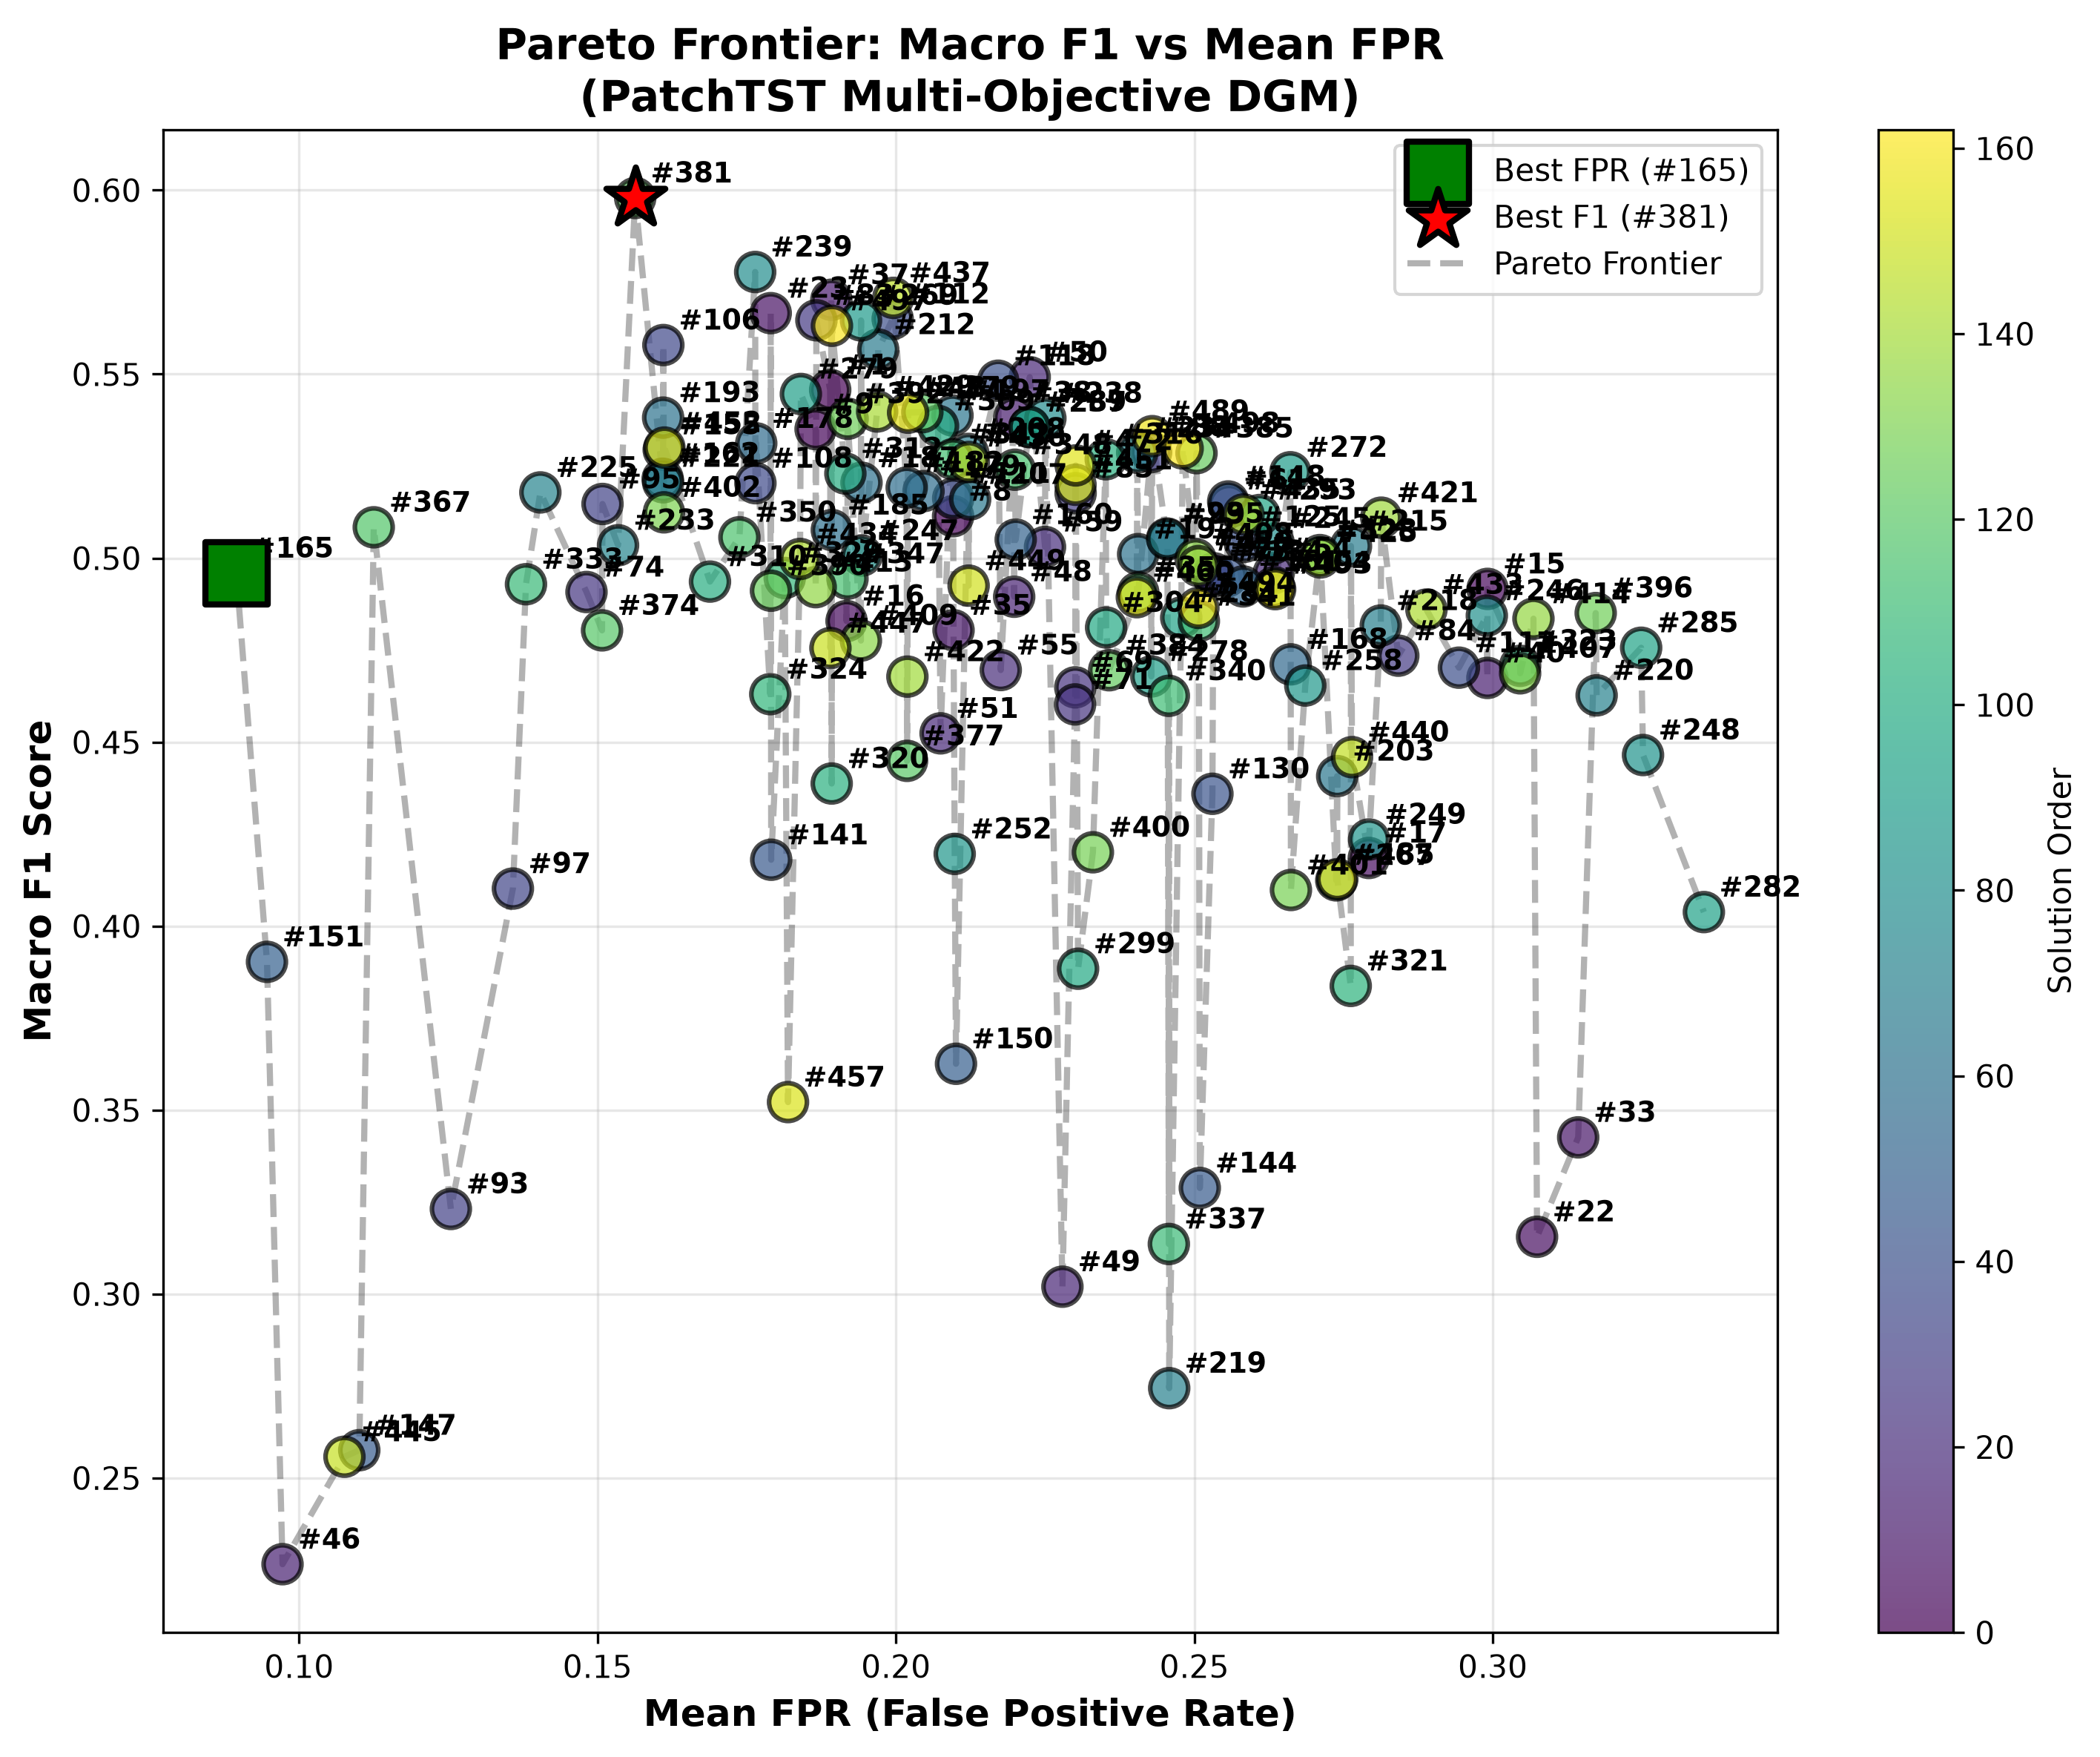
\includegraphics[width=0.45\textwidth]{figures/phase3_pareto_f1_vs_fpr.png}
\caption{Phase~3 Pareto frontier: macro-F1 vs. mean-FPR trade-off.
Trial~\#381 ($\alpha_{\text{FL}}{=}0.866$, $\gamma{=}1.156$)
achieves macro-F1=0.776 with controlled FPR=0.080.
448/500 trials (89.6\%) are Pareto-optimal.}
\label{fig:phase3_pareto}
\end{figure}

\begin{figure}
\centering
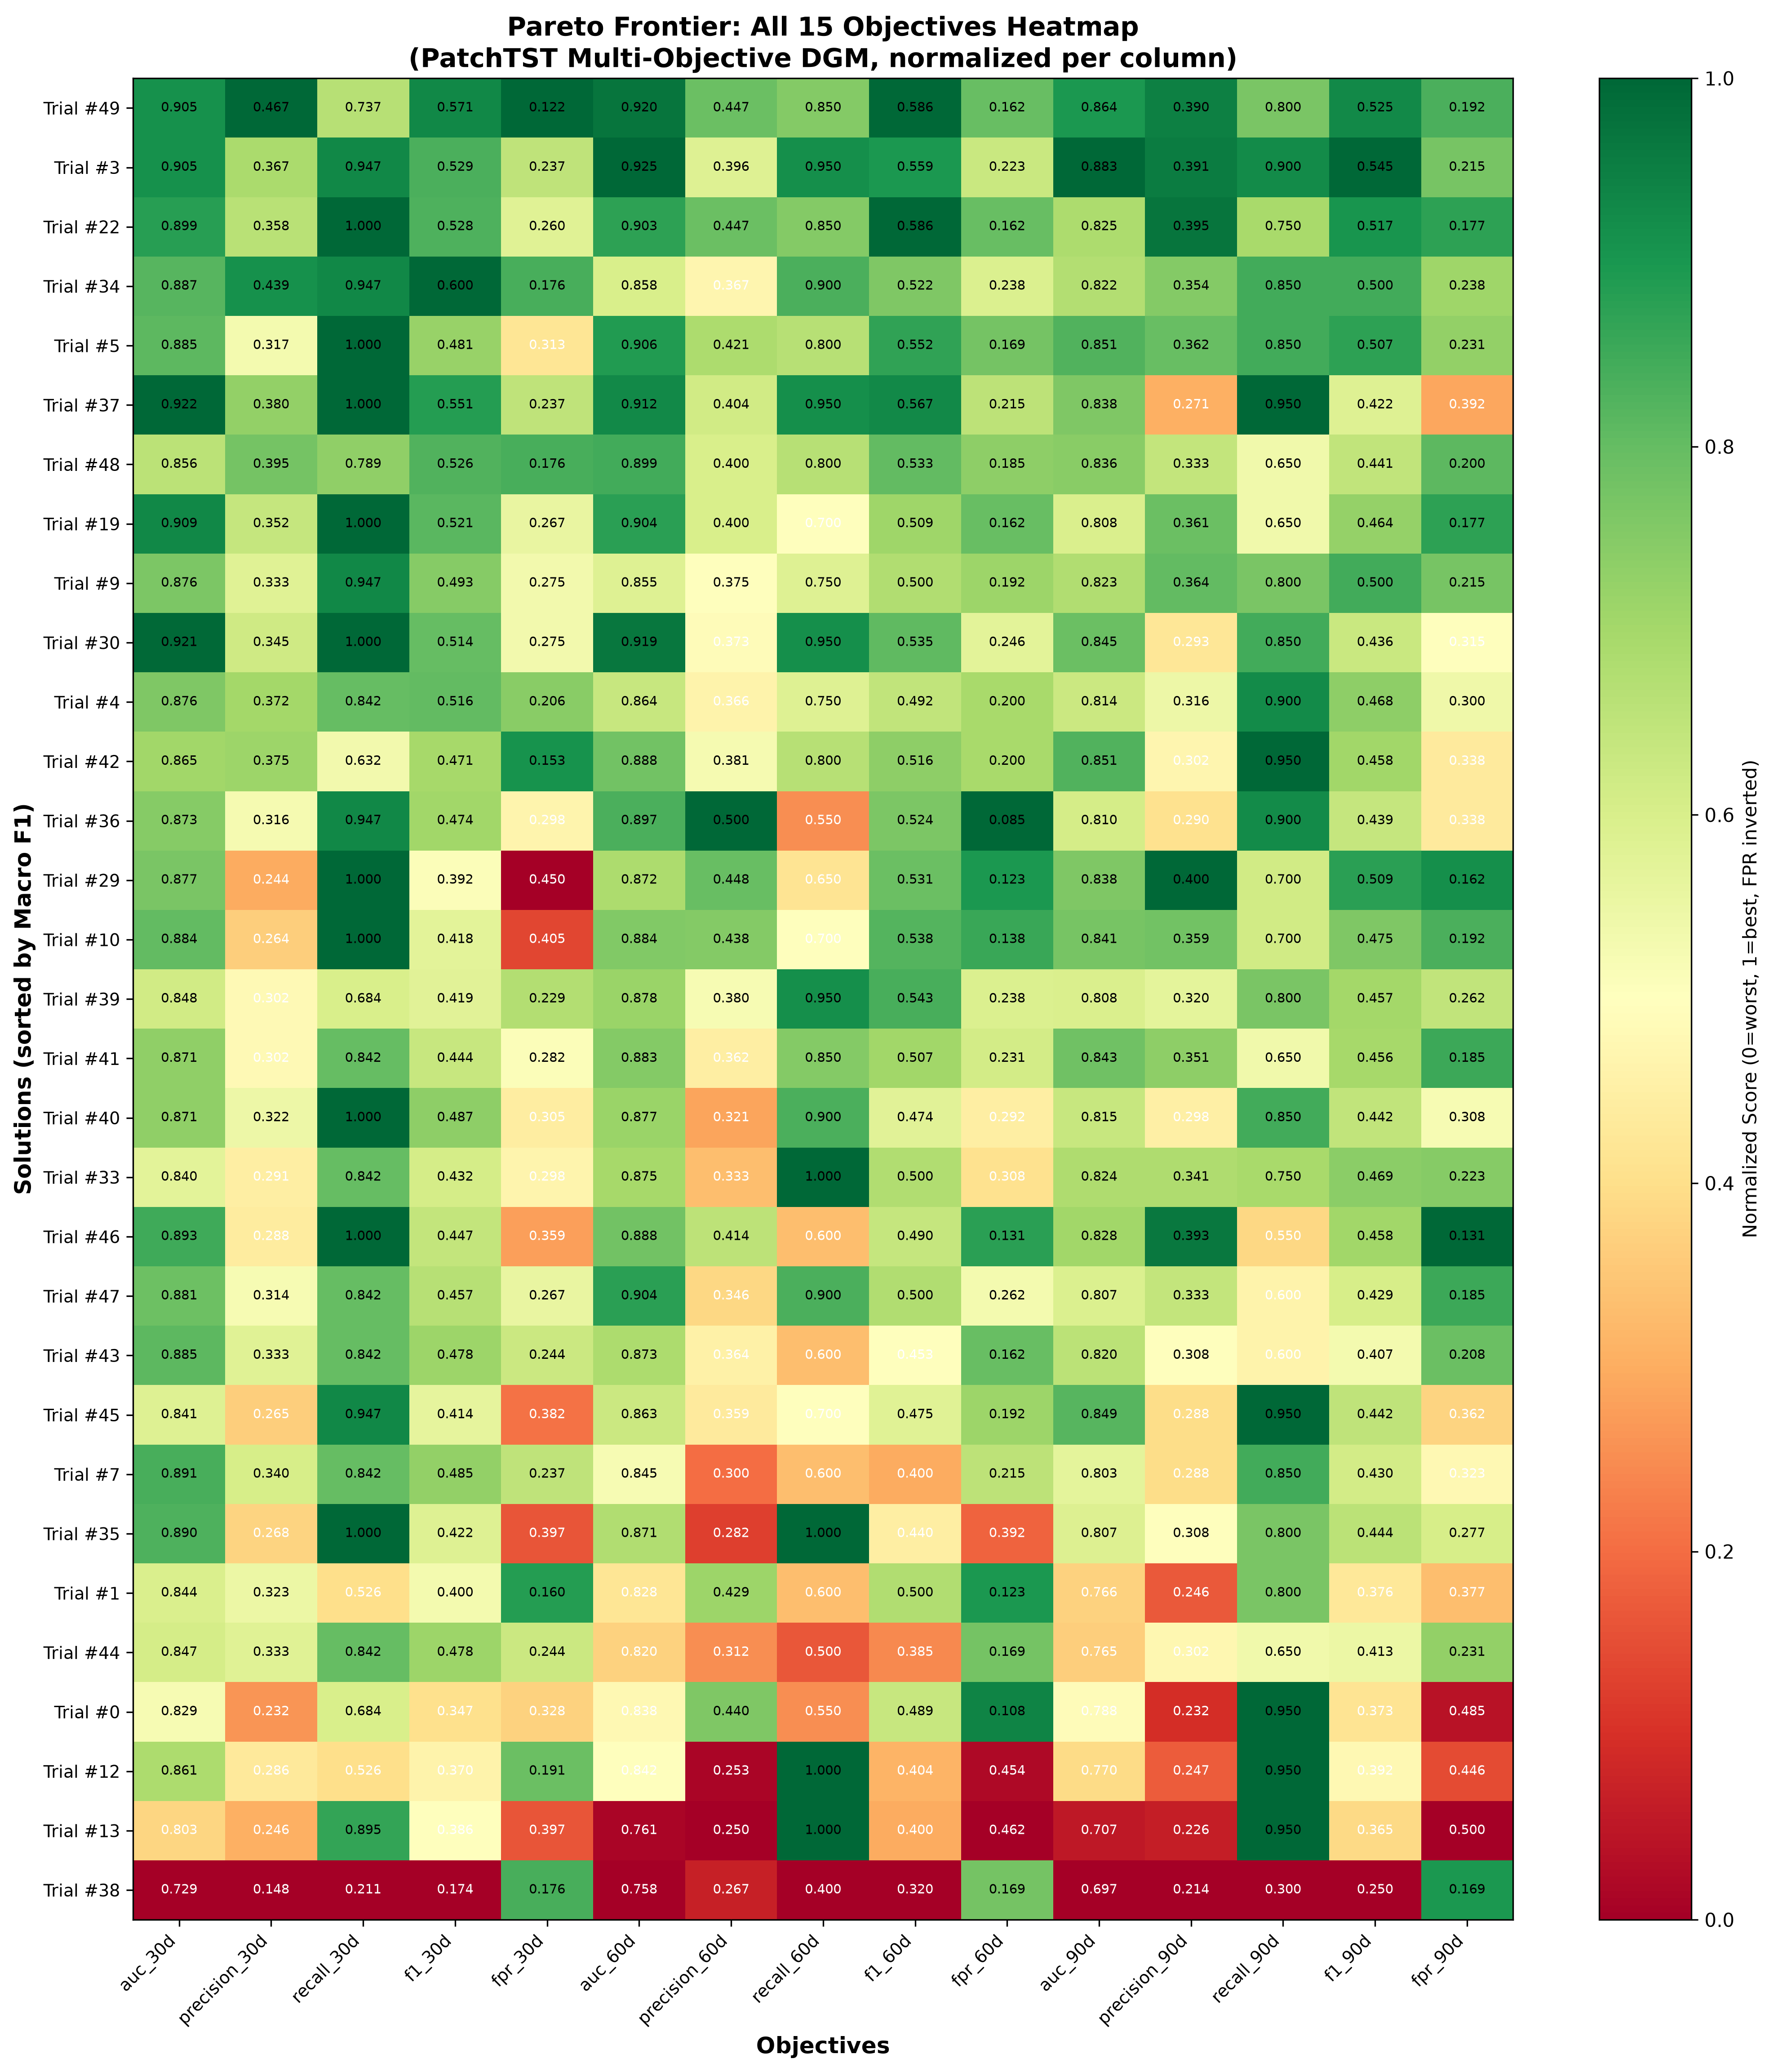
\includegraphics[width=0.45\textwidth]{figures/pareto_objectives_heatmap.png}
\caption{Phase~3 multi-objective contribution heatmap (early iterations).
Each row represents a trial, each column an objective
(AUC/Precision/Recall/F1/FPR $\times$ 3 horizons = 15 objectives).
Colour intensity indicates relative performance.
The heatmap demonstrates that each trial contributes to different
objective subsets, with no single trial dominating all 15 dimensions
simultaneously---validating the necessity of multi-objective
Pareto optimization over single-objective approaches.}
\label{fig:phase3_heatmap}
\end{figure}

\subsection{Phase~4: Architecture 2D DGM}

\subsubsection{Pareto Frontier (3 Non-Dominated Solutions)}

Table~\ref{tab:v03_pareto} shows the Pareto frontier from the
initial Phase~4 run (200~iterations).
Trial~\#1 achieves the best macro-F1 of \textbf{0.773} with
patch\_len=26, stride=16, an overlap of 62\%.
The ratio $s / L_p = 16/26 \approx 0.615$ closely approximates
$\varphi^{-1} \approx 0.618$, suggesting a naturally balanced
patch granularity for 90-day pump sequences.

\begin{table}
\centering
\caption{Phase~4 Pareto frontier (3 non-dominated solutions).}
\label{tab:v03_pareto}
\small
\renewcommand{\arraystretch}{1.05}
\setlength{\tabcolsep}{4pt}
\begin{tabular}{lrrrrrr}
\toprule
Trial & $L_p$ & $s$ & Overlap & macro-F1 & mean-FPR \\
\midrule
\#0 & 17 & 8  & 47\% & 0.721 & 0.048 \\
\rowcolor{green!10}
\textbf{\#1} & \textbf{26} & \textbf{16} & \textbf{62\%} & \textbf{0.773} & \textbf{0.033} \\
\#2 & 11 & 7  & 64\% & 0.735 & 0.030 \\
\bottomrule
\end{tabular}
\end{table}

\begin{figure}
\centering
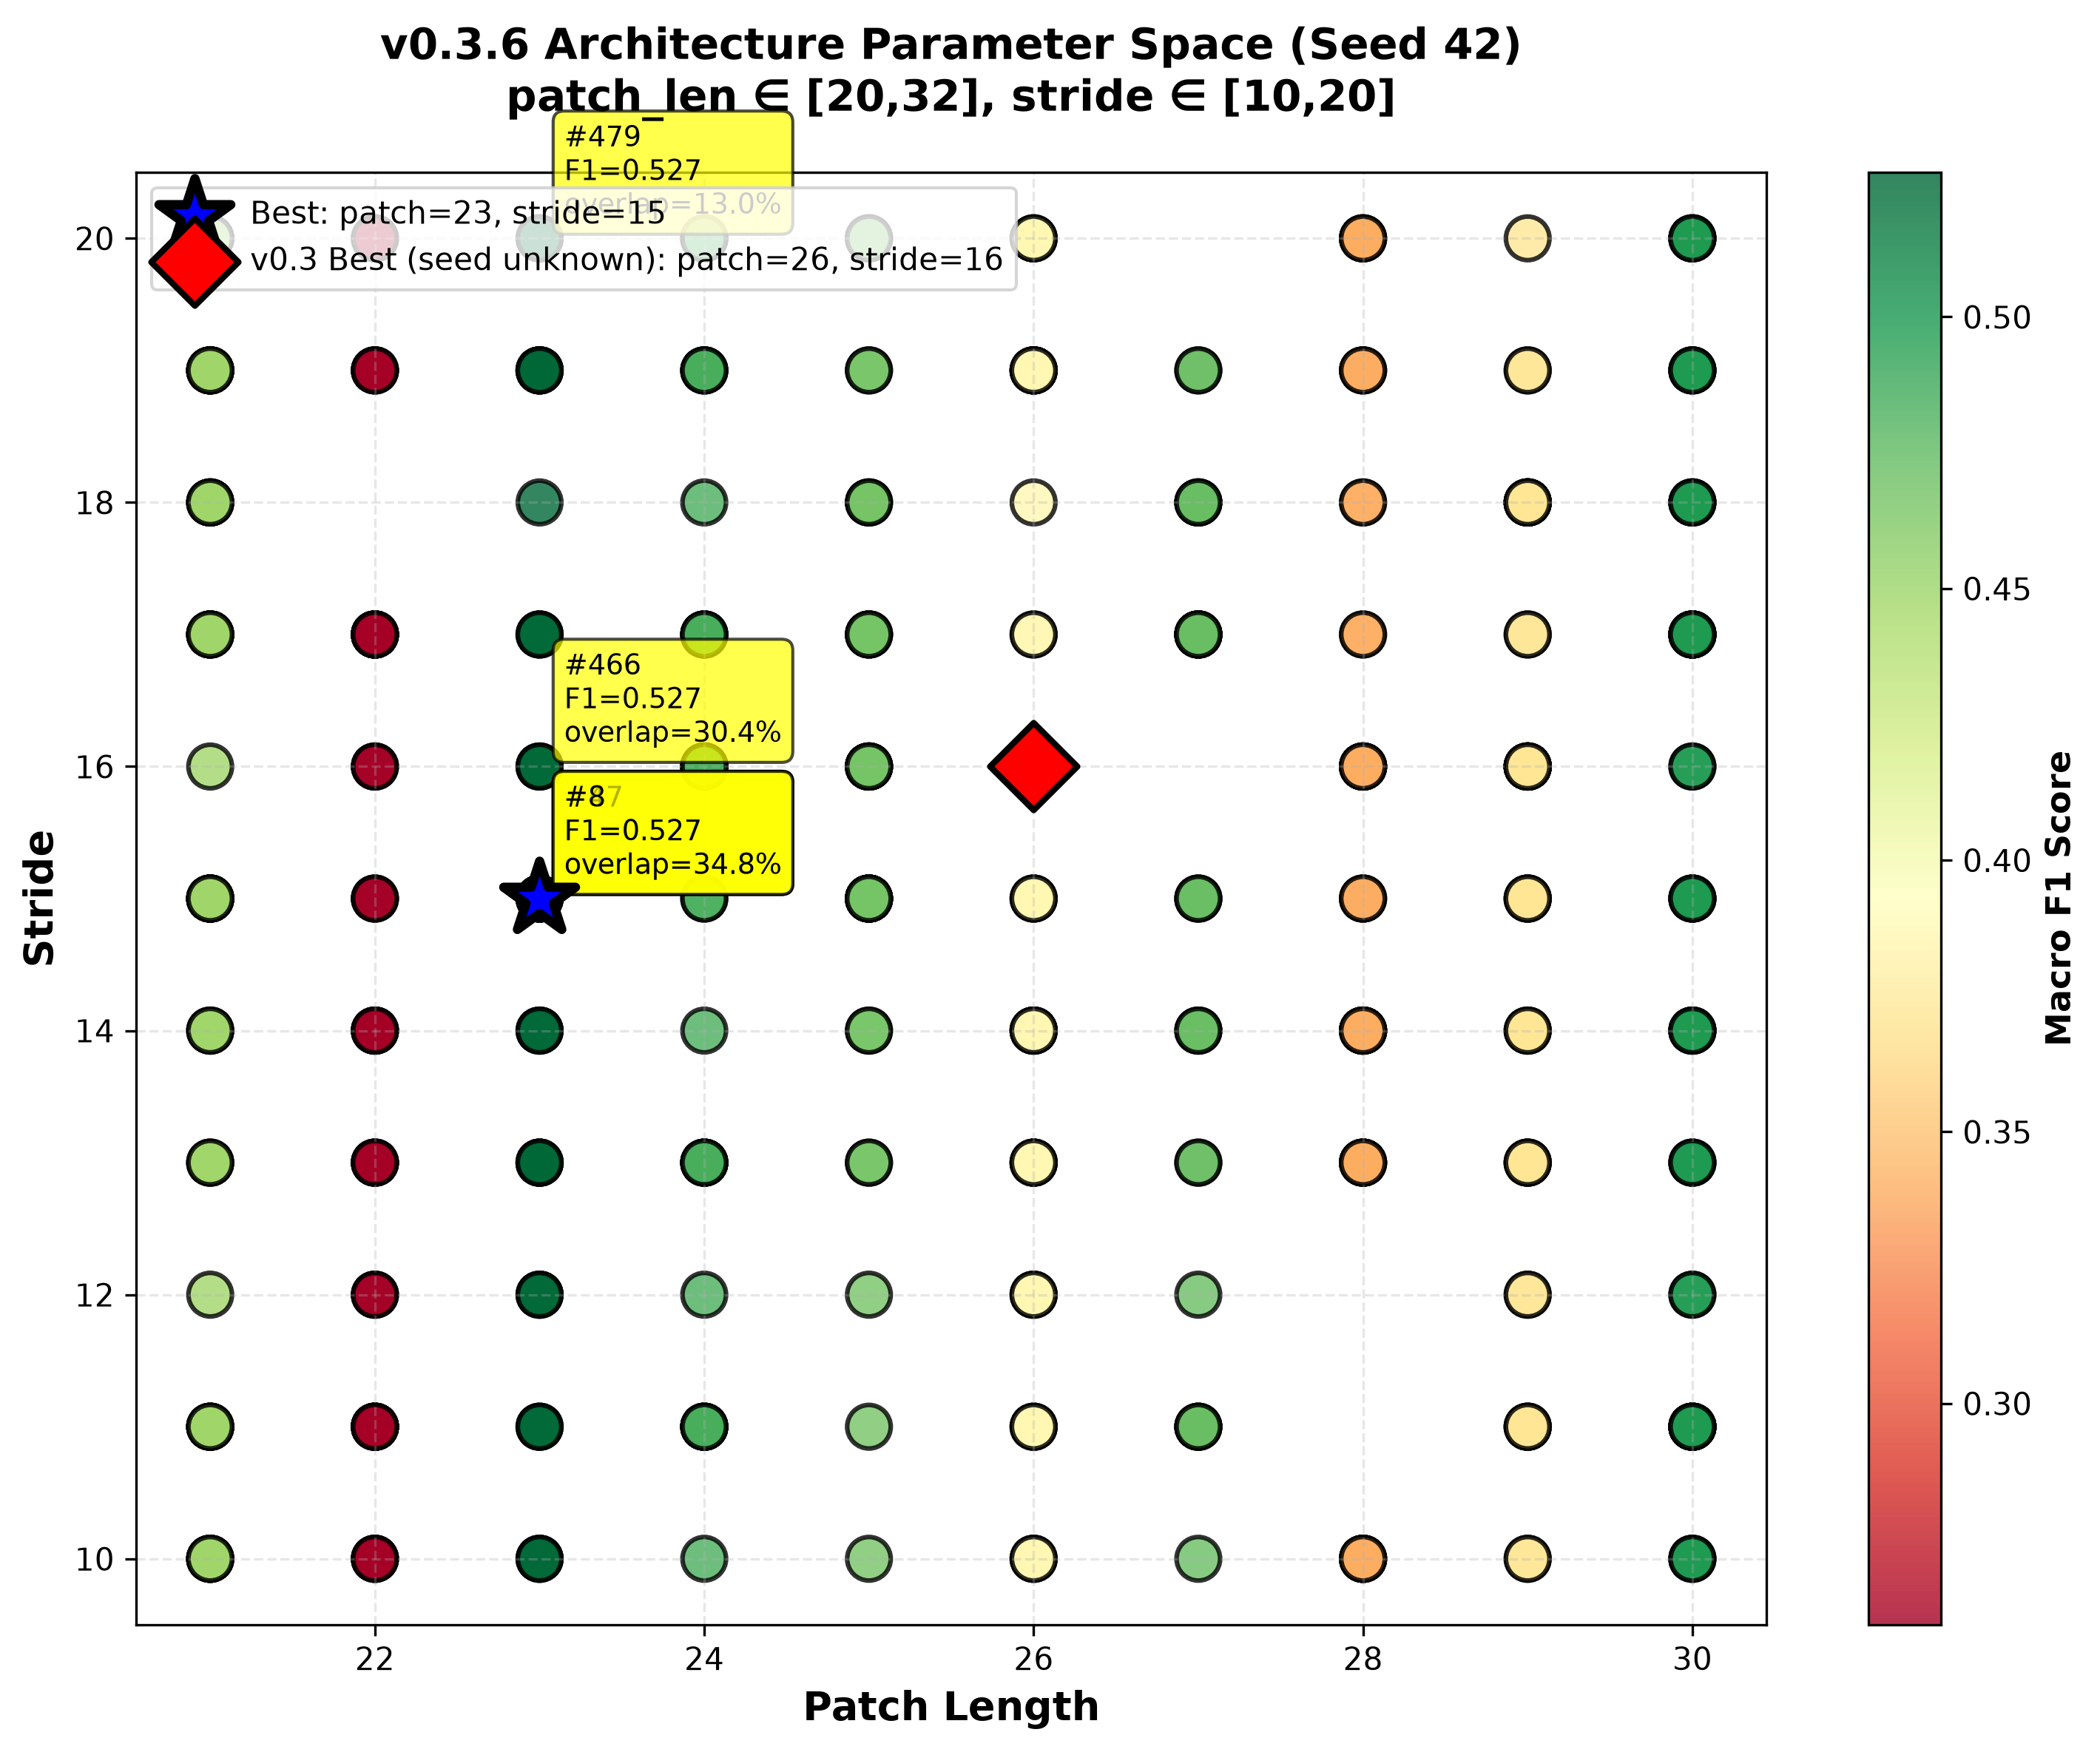
\includegraphics[width=0.45\textwidth]{figures/phase4_architecture_space.png}
\caption{Phase~4 2D architecture space: patch\_len ($L_p$) vs. stride ($s$).
The Pareto frontier (green) concentrates around 60--64\% overlap,
with Trial~\#1 ($L_p{=}26$, $s{=}16$, overlap=62\%) achieving
macro-F1=0.773. Ratio $s/L_p \approx 0.615$ closely approximates
$\varphi^{-1} \approx 0.618$ (golden ratio).}
\label{fig:phase4_arch}
\end{figure}

\subsection{Joint optimization: 4D to 8D}
\label{subsec:joint_results}

Table~\ref{tab:joint_results} compares the three structured
joint optimization experiments.
Macro-F1 improves monotonically from 4D to 8D
yet all three fall substantially below the stepwise Phase~3 best (0.776).

\begin{table}
\centering
\caption{Joint optimization macro-F1 progression (best solutions).}
\label{tab:joint_results}
\small
\renewcommand{\arraystretch}{1.05}
\setlength{\tabcolsep}{3pt}
\begin{tabular}{llrrrr}
\toprule
\textbf{Dims} & \textbf{Iters} & \textbf{Pareto} & \textbf{macro-F1} & \textbf{$\Delta$ vs 4D} \\
\midrule
4D & 1000 & 20.5\% & 0.614 & --- \\
6D & 2000 & 27.7\% & 0.642 & +4.6\% \\
\rowcolor{green!10}
\textbf{8D} & 3000 & 20.6\% & \textbf{0.656} & +6.8\% \\
\bottomrule
\end{tabular}
\end{table}

The joint 8D best (Trial~\#1891:
$L_p{=}26$, $s{=}16$, $r{=}16$, $\alpha_L{=}47$,
$\alpha_{\text{FL}}{=}0.775$, $\gamma{=}0.607$,
$w_n{=}2.501$, $w_a{=}2.225$)
achieved macro-F1~=~0.656, 12.0 percentage points below
the stepwise Phase~3 best, validating the phased approach.

Figure~\ref{fig:v021v022_pareto} shows the Pareto frontiers of v0.2.1
and v0.2.2, illustrating how the trade-off curve improves as more
dimensions are jointly optimised.

\begin{figure}
\centering
\begin{subfigure}[t]{0.48\columnwidth}
  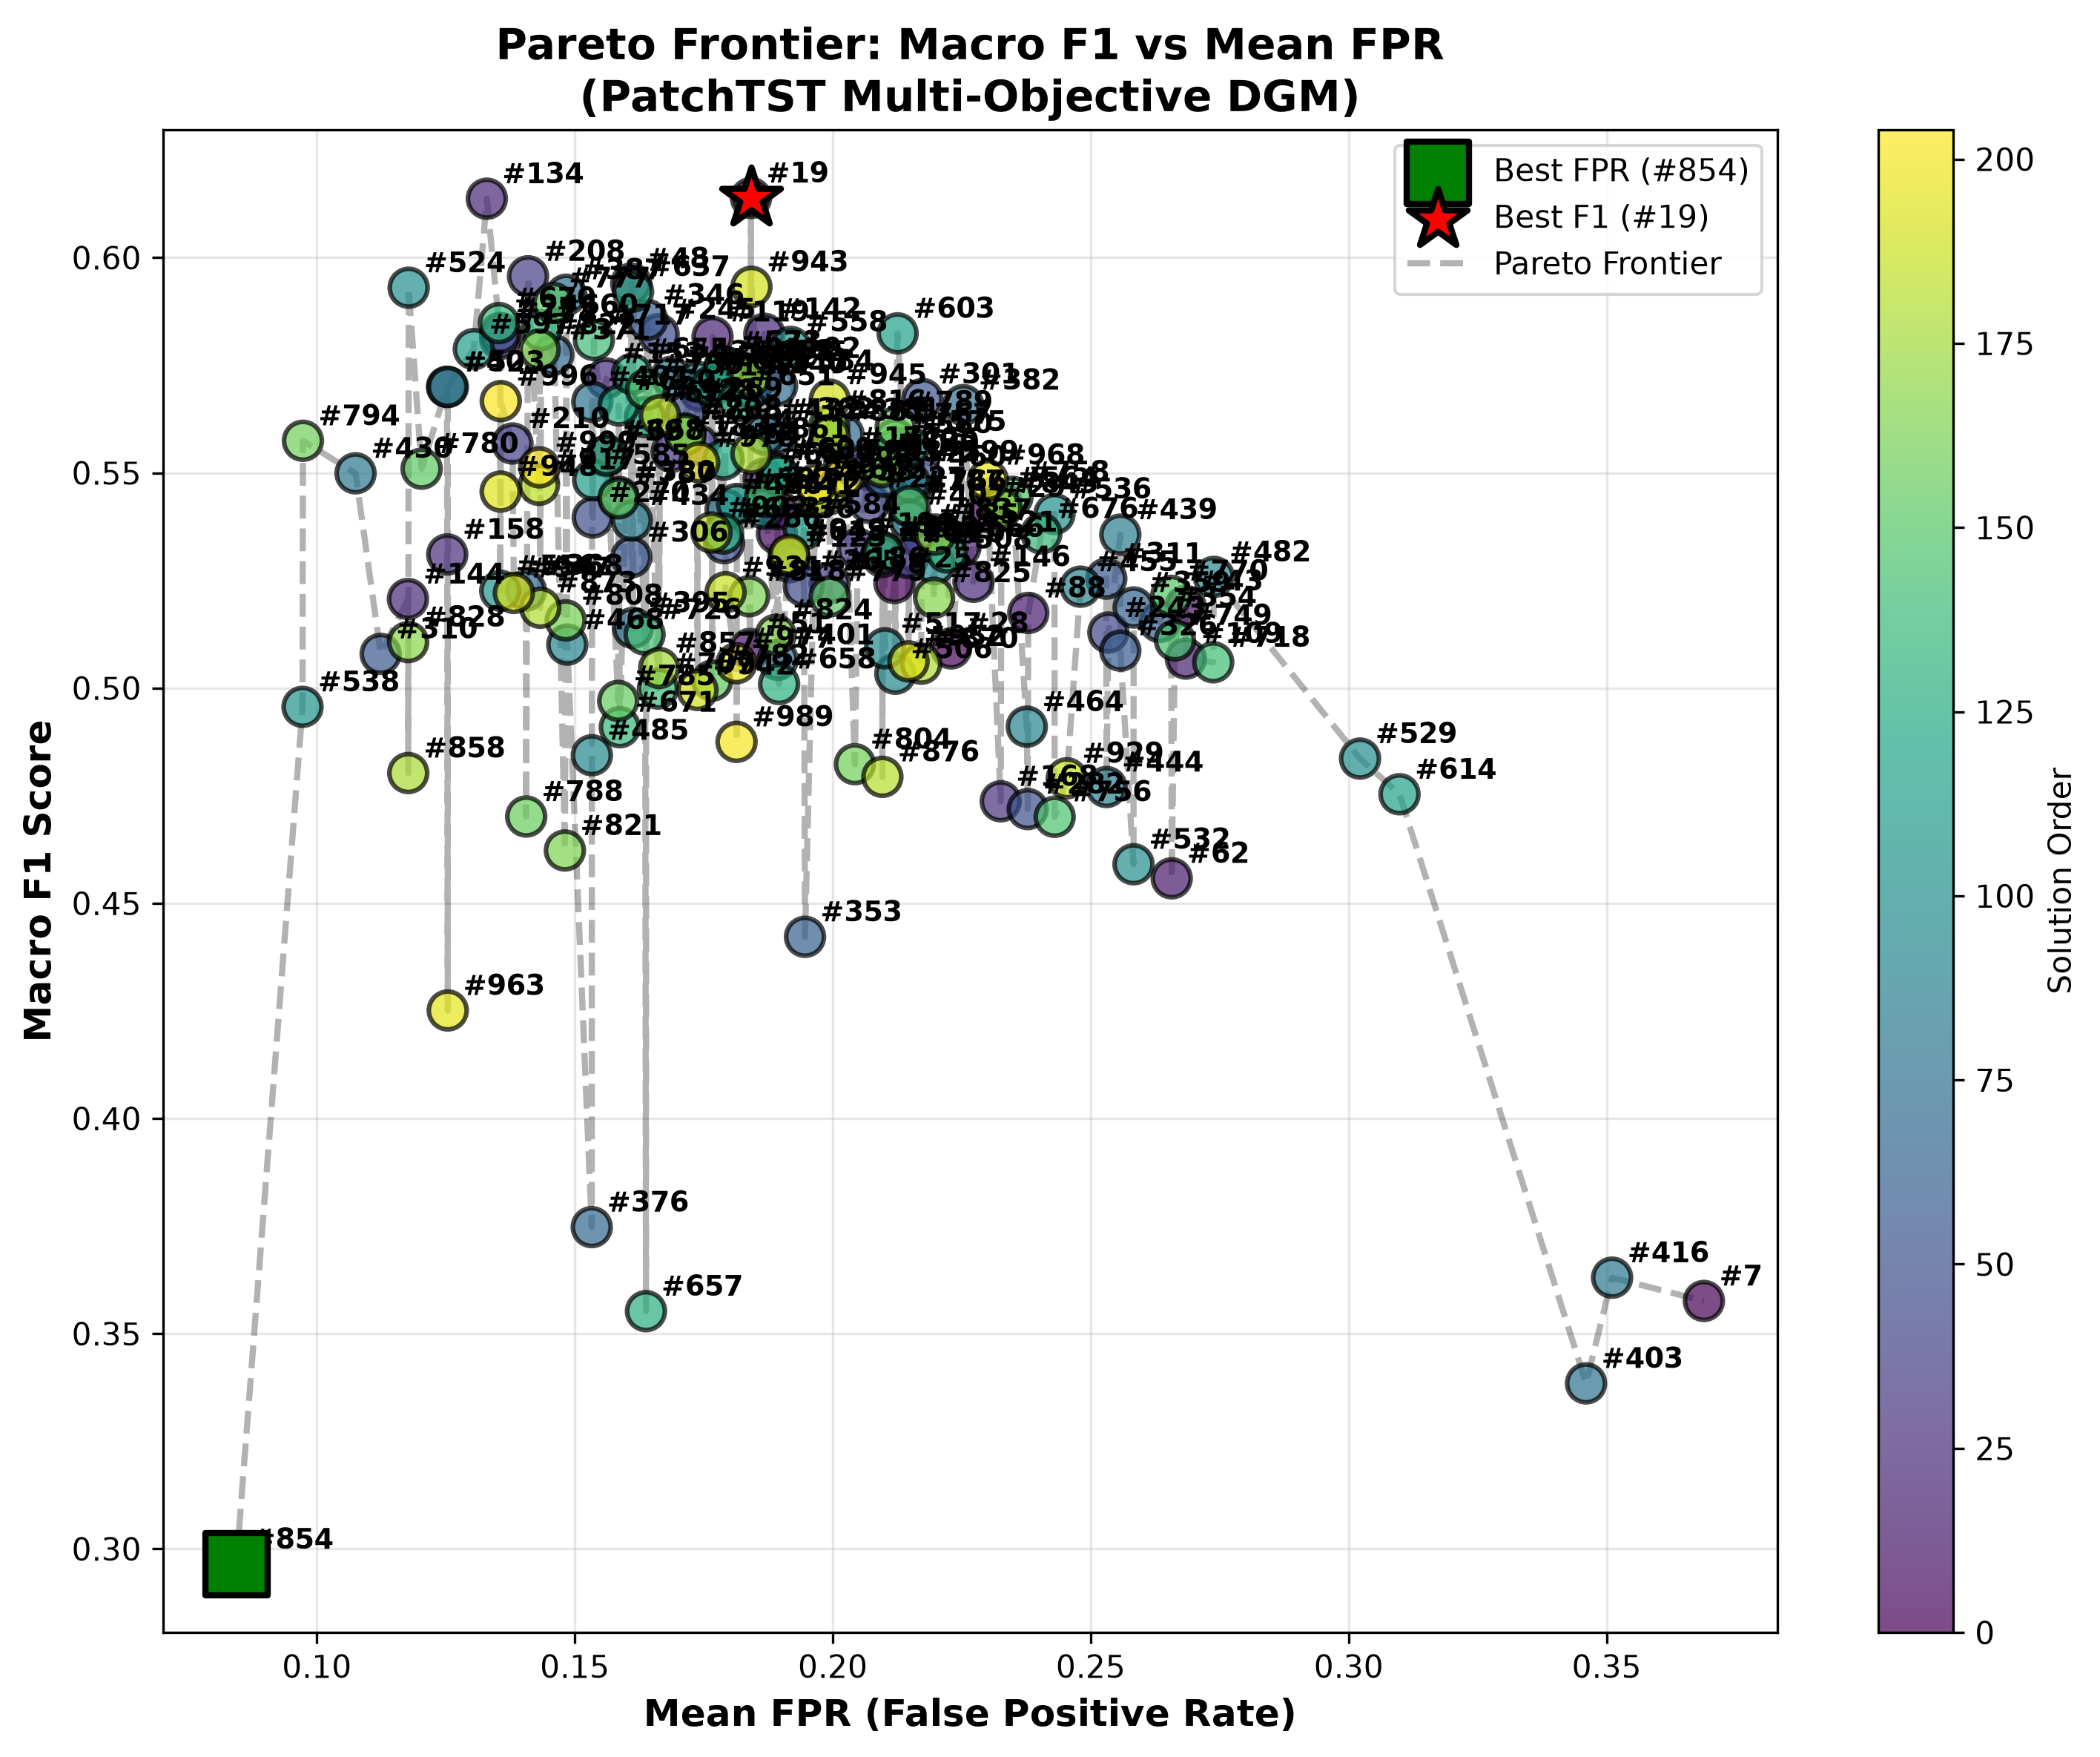
\includegraphics[width=\linewidth]{figures/v021_pareto_f1_vs_fpr.png}
  \caption{Joint (4D): macro-F1~=~0.614, Pareto 20.5\%}
  \label{fig:v021_pareto}
\end{subfigure}\hfill
\begin{subfigure}[t]{0.48\columnwidth}
  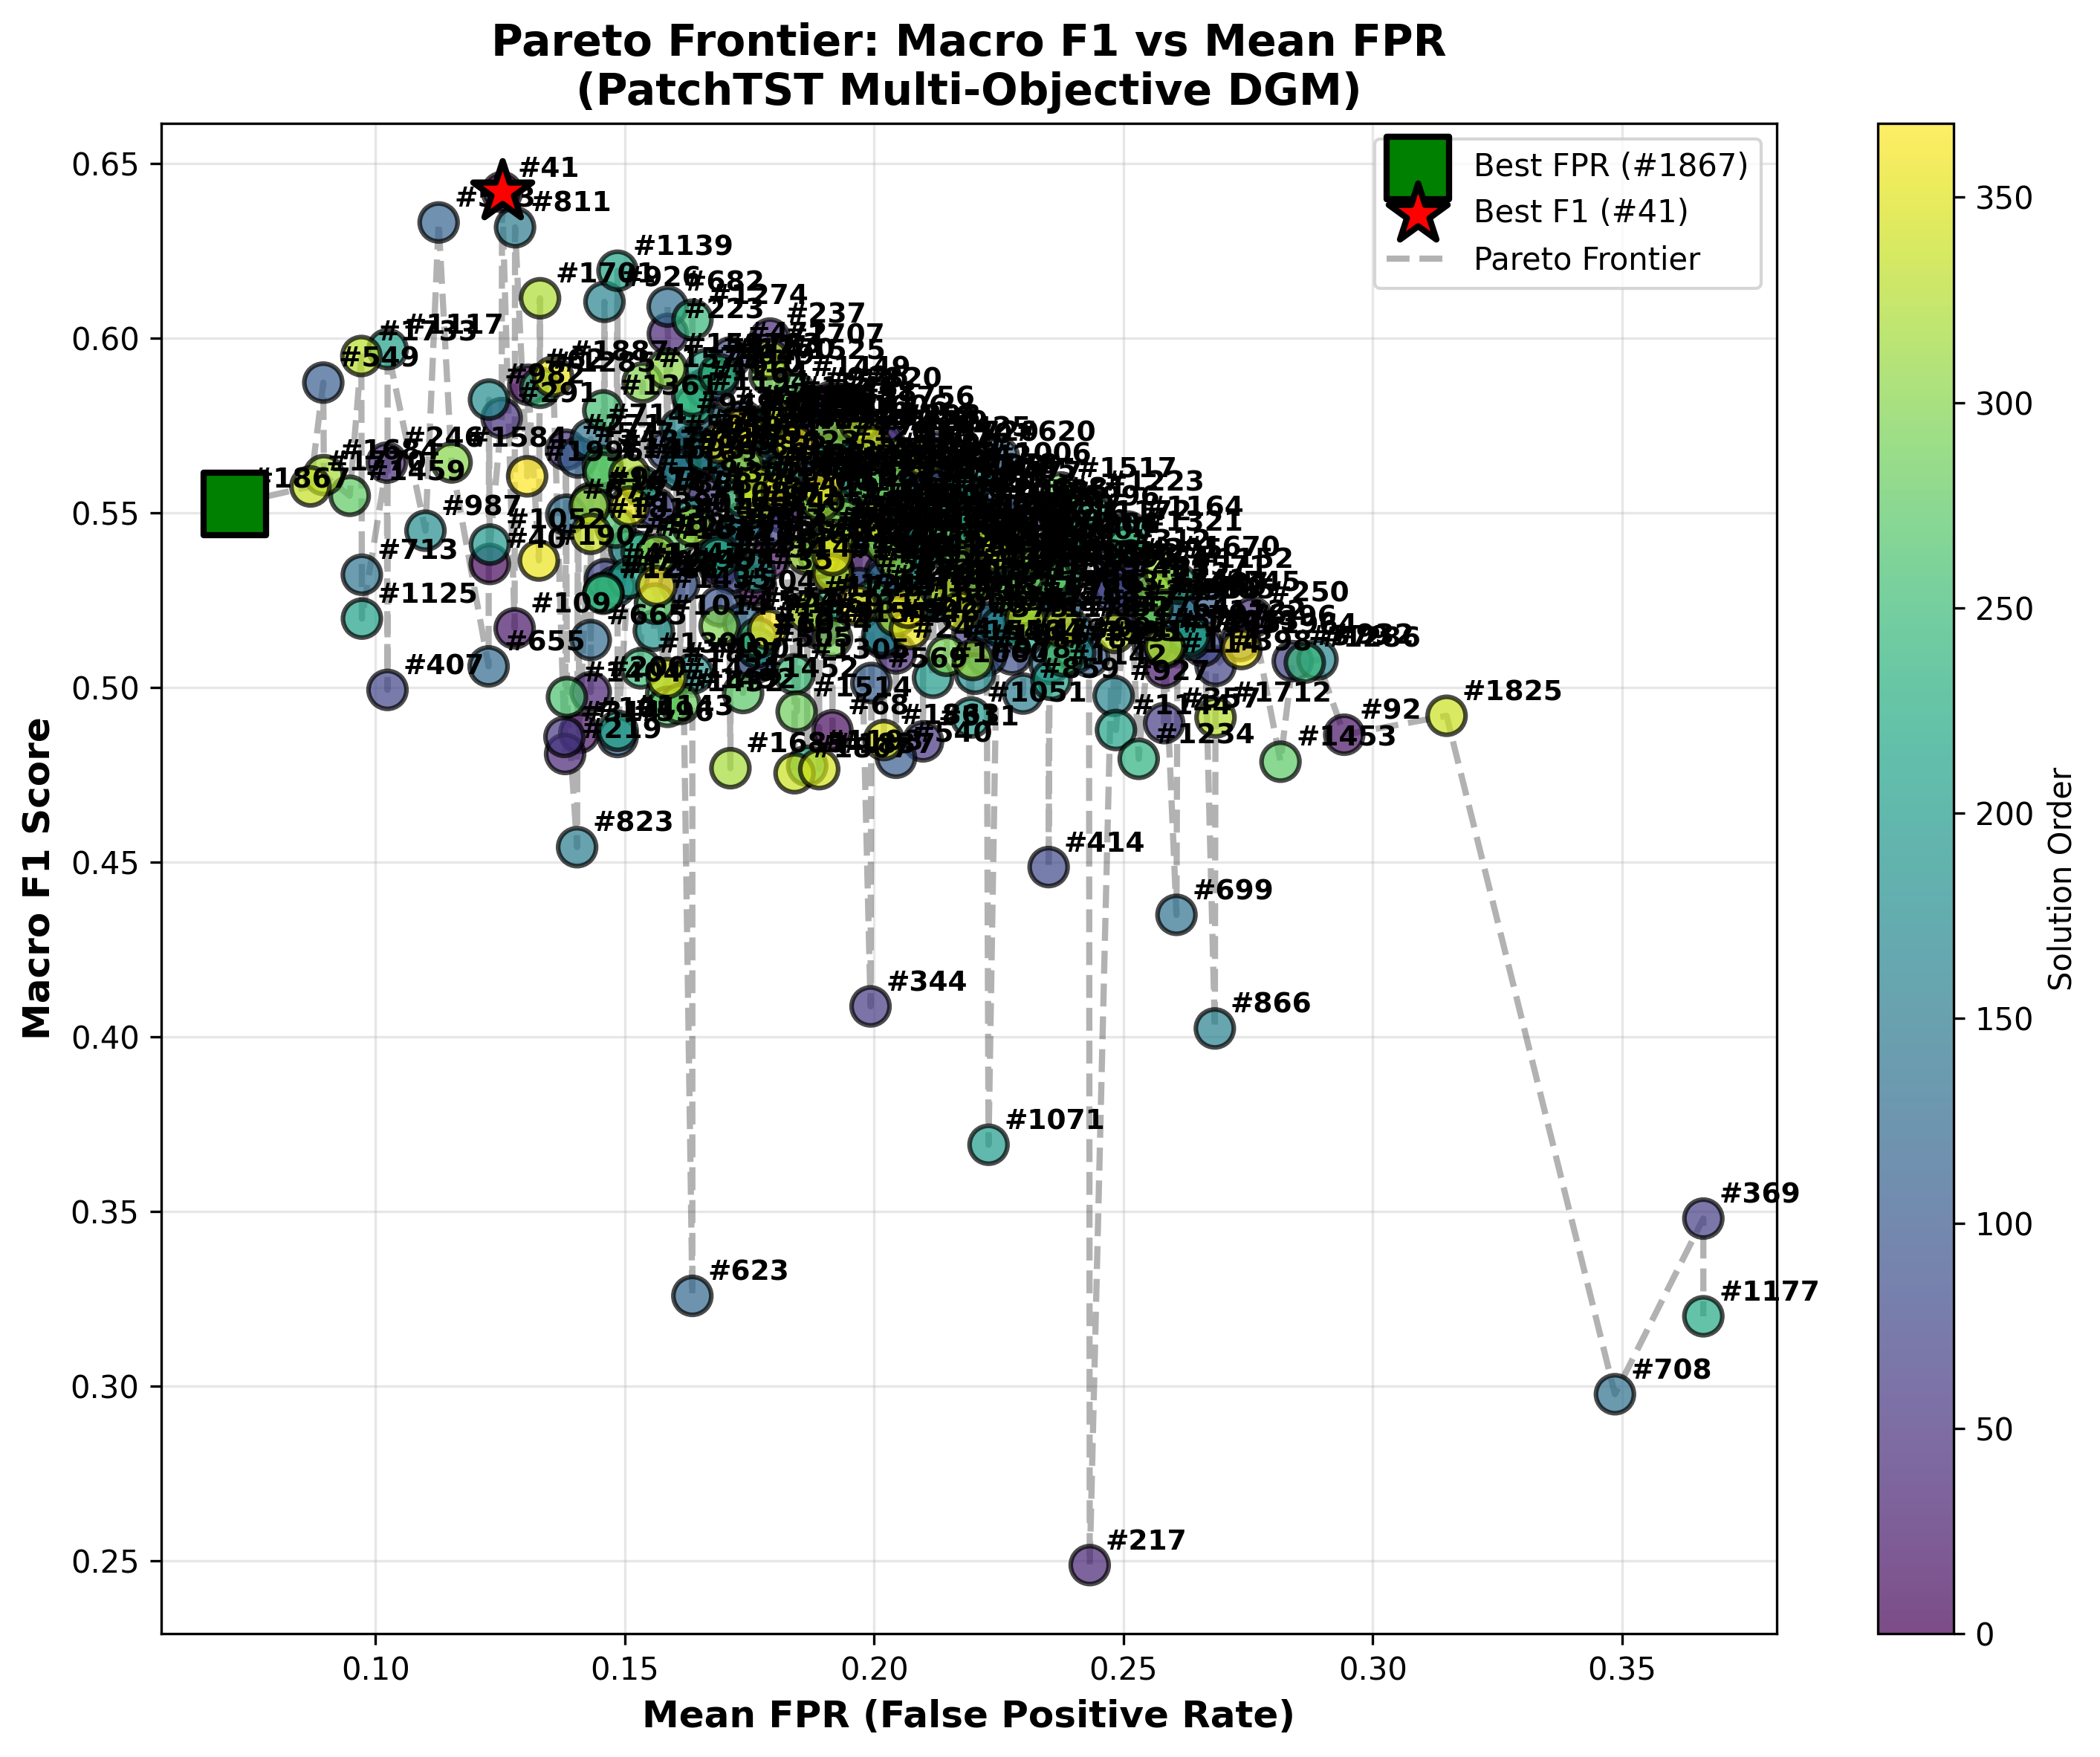
\includegraphics[width=\linewidth]{figures/v022_pareto_f1_vs_fpr.png}
  \caption{Joint (6D): macro-F1~=~0.642, Pareto 27.7\%}
  \label{fig:v022_pareto}
\end{subfigure}
\caption{Pareto frontier progression: Joint (4D Focal Loss + Class Weights)
vs.\ Joint (6D Architecture + LoRA + Focal Loss, Class Weights fixed).
Expanding from 4D to 6D shifts the frontier rightward and upward,
gaining +4.6\% macro-F1 while the 6D frontier achieves higher
Pareto-optimal rate (27.7\% vs.\ 20.5\%).}
\label{fig:v021v022_pareto}
\end{figure}

\begin{figure}
\centering
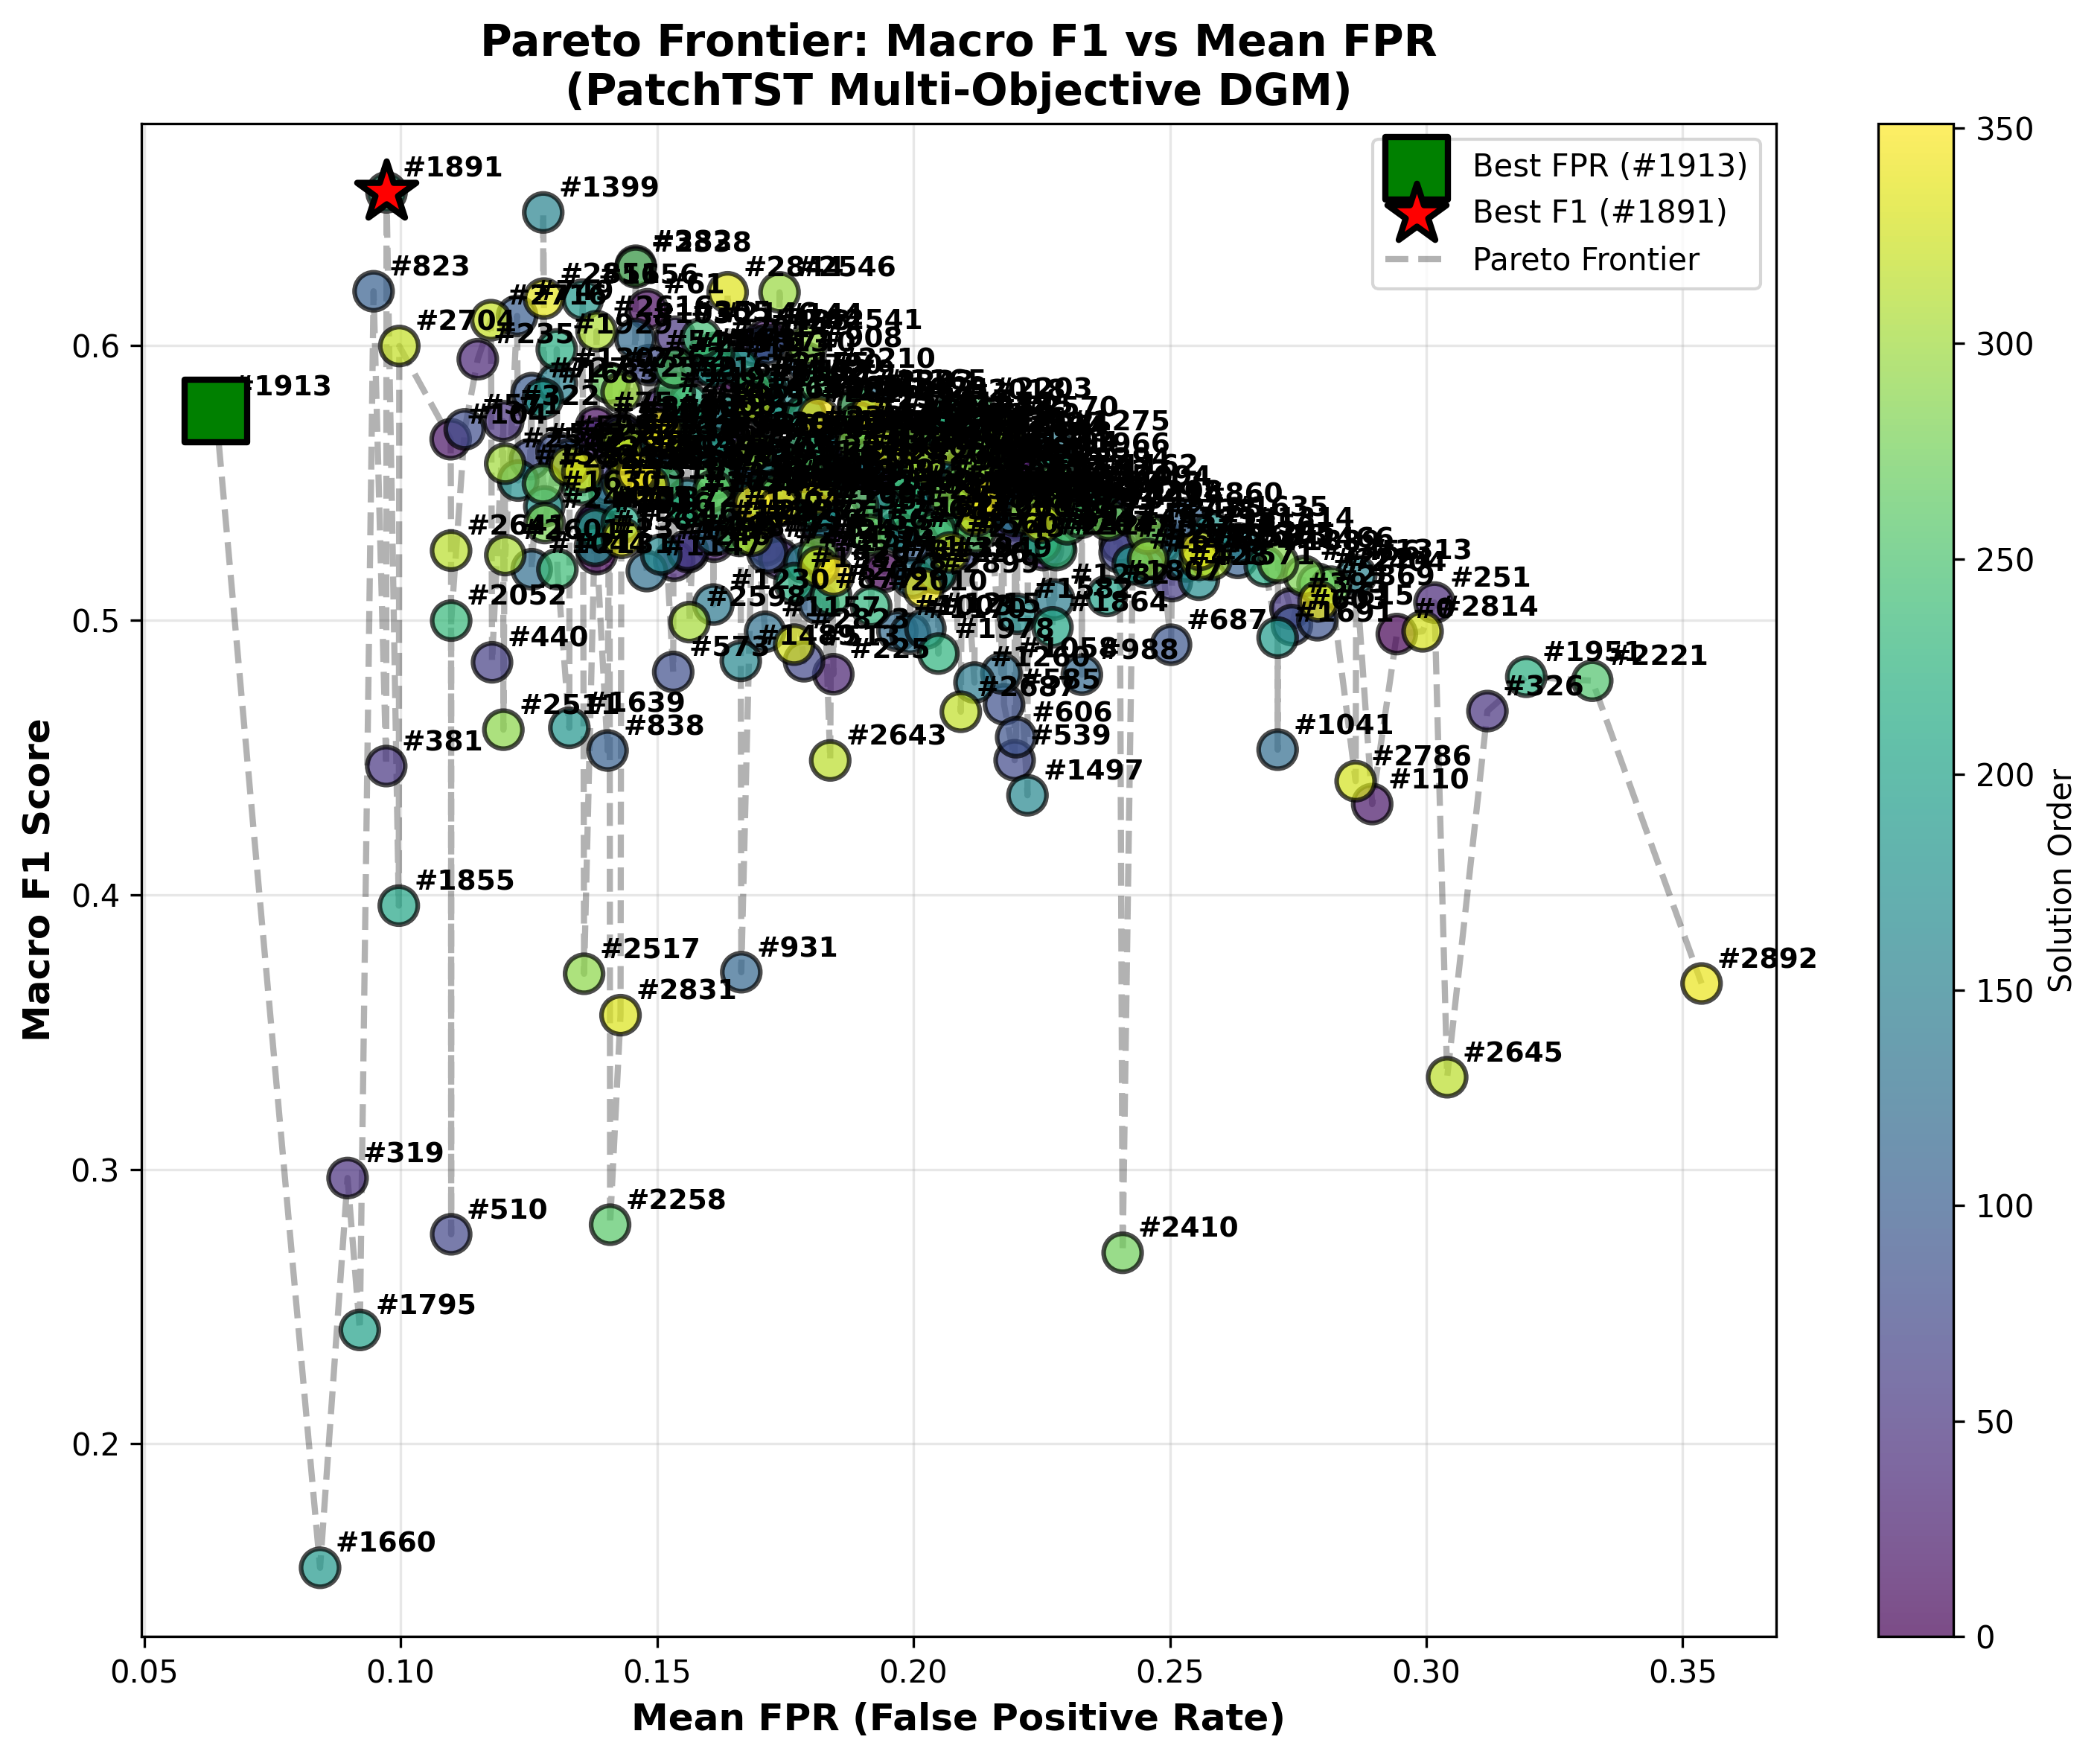
\includegraphics[width=0.45\textwidth]{figures/v023_pareto_f1_vs_fpr.png}
\caption{Joint (8D) Pareto frontier: macro-F1 vs.\ mean-FPR.
352 non-dominated solutions from 3000 iterations.
Best macro-F1~=~0.656 (Trial~\#1891).
The 12-point gap to Phase~3 stepwise (0.776) confirms that
joint optimization in high-dimensional space cannot substitute
for the stepwise decomposition.}
\label{fig:v023_pareto}
\end{figure}

\begin{figure*}
\centering
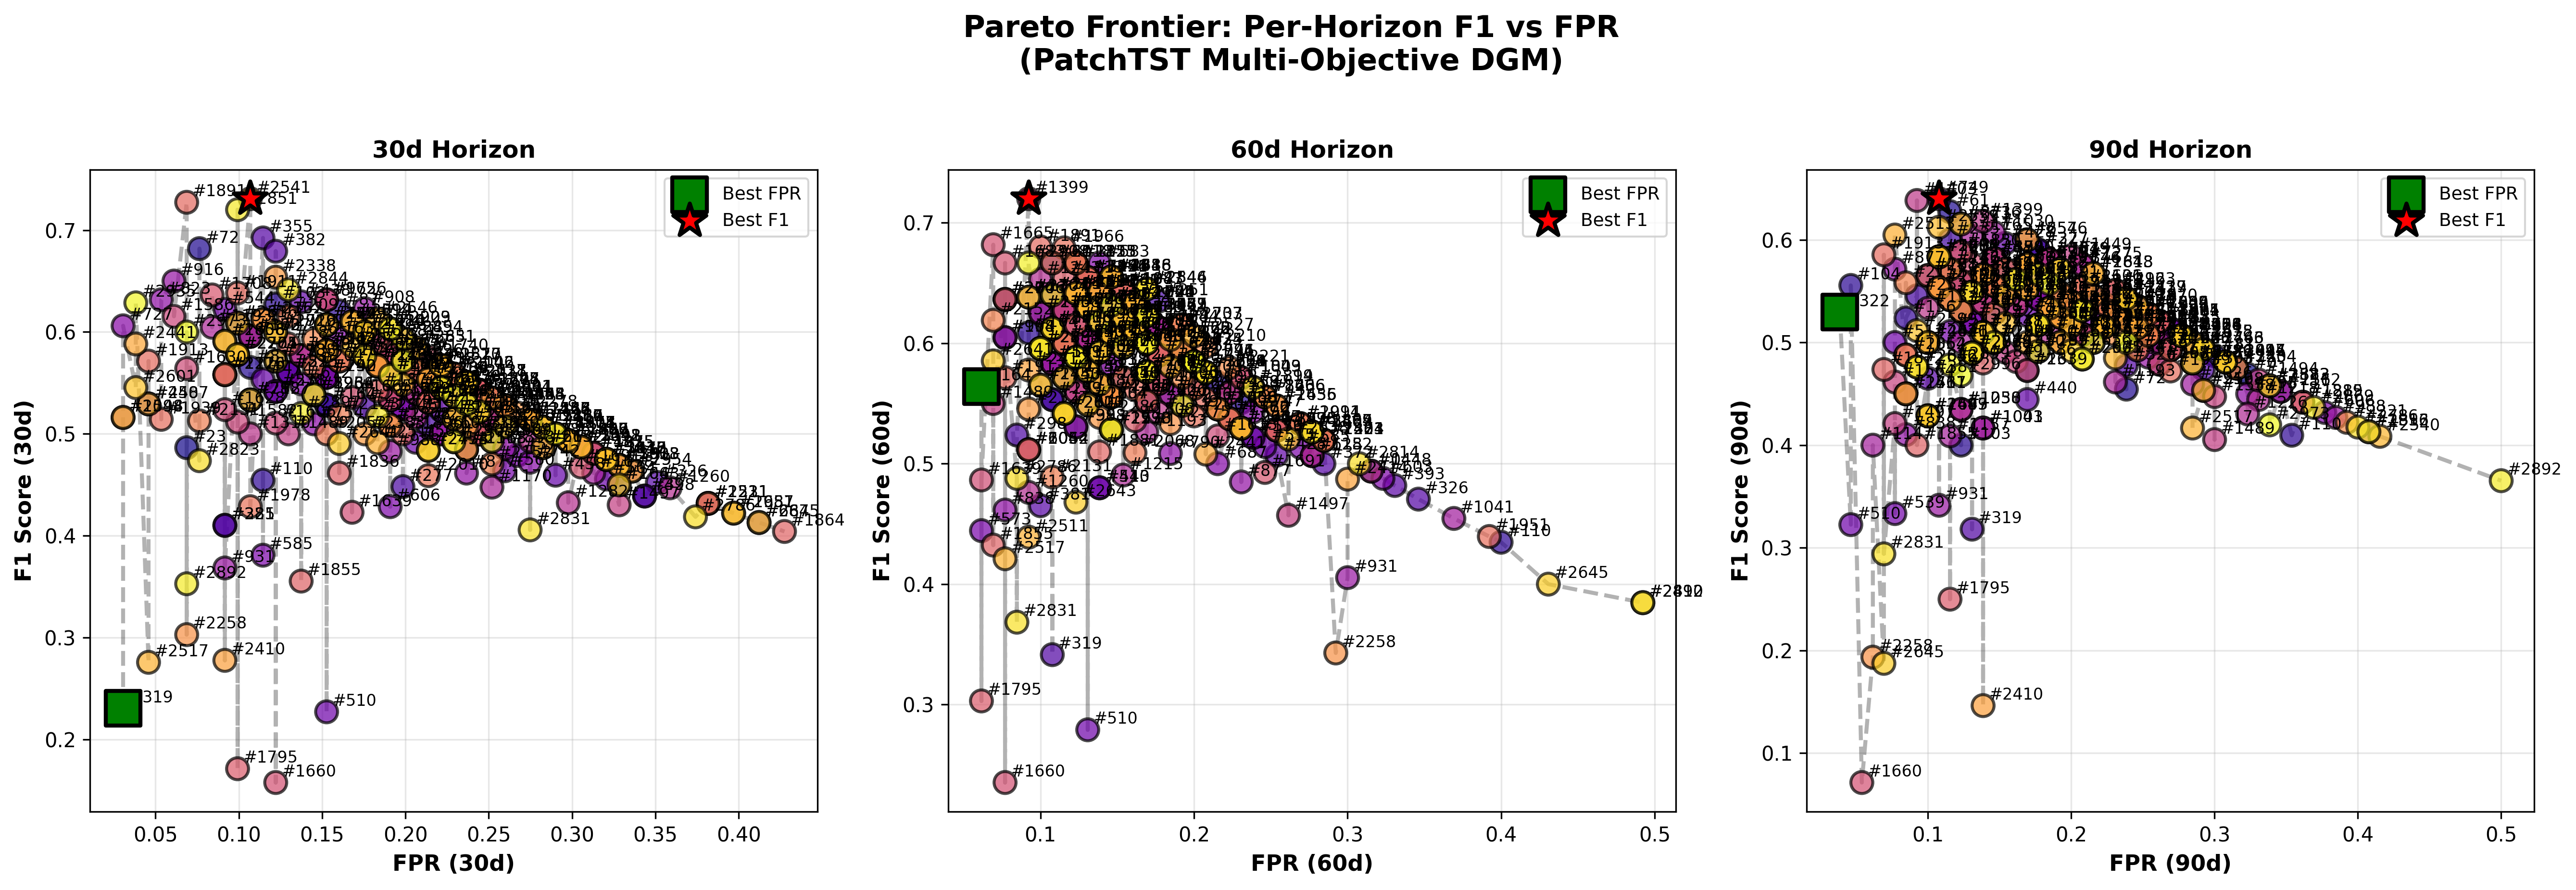
\includegraphics[width=0.92\textwidth]{figures/v023_per_horizon_f1_fpr.png}
\caption{Joint (8D) per-horizon Pareto frontiers: F1 vs.\ FPR at 30d, 60d, and 90d.
Best per-horizon F1: 30d~=~0.731, 60d~=~0.720, 90d~=~0.640.
The 90d frontier (rightmost) shows wider scatter and lower peak F1,
confirming that 8D joint optimization amplifies horizon degradation
(30d$\to$90d: $-$12.4\%) compared to the stepwise approach ($-$4.6\%).
The 30d and 60d frontiers are denser and better-defined,
suggesting that NSGA-II prioritises short-horizon objectives over
the harder long-horizon ones when averaging across all 15.}
\label{fig:v023_per_horizon}
\end{figure*}

\textbf{Empirical findings from the joint experiments.}

\begin{enumerate}[leftmargin=*,topsep=2pt,itemsep=1pt]
  \item \textbf{LoRA $\alpha_L/r \approx 2.9$ is a robust scaling law.}
        The ratio is stable at $2.7$--$2.9$ across
        2D, 6D, and 8D contexts
        ($53/19{=}2.79$ in v0.3.6.3;
        $54/20{=}2.70$ in v0.2.2;
        $47/16{=}2.94$ in v0.2.3 best).
        Setting $\alpha_L = 3r$ as a fixed rule and tuning only $r$
        is equivalent to a 2D LoRA search.

  \item \textbf{Diminishing returns of dimension expansion.}
        Each 2D expansion yields approximately half the preceding gain:
        4D$\to$6D: $+4.6\%$; 6D$\to$8D: $+2.2\%$.
        The residual 12.0-point gap to the stepwise best
        cannot be closed by further dimension expansion.

  \item \textbf{Cross-component interactions are weak.}
        Spearman correlations between parameters in the top-100
        Pareto solutions (v0.2.3) are $|{\rho}| < 0.3$ for all
        cross-component pairs except the intra-LoRA coupling
        ($\alpha_L$--$r$: $\rho{=}0.98$).
        Parameter interactions are mostly local (within one component)
        rather than global, supporting the stepwise structural prior.

  \item \textbf{Horizon degradation is amplified by joint optimization.}
        F1 from 30d to 90d falls by 12.4\% under joint optimization
        vs.~4.6\% under stepwise (Figure~\ref{fig:v023_per_horizon}).
        NSGA-II averaging across all 15 objectives may overfit
        short-horizon patterns at the expense of long-horizon ones.

  \item \textbf{Pareto optimality rate decreases with dimensionality.}
        The fraction of Pareto-optimal trials drops from 27.7\% (6D)
        to 20.6\% (8D) despite a 50\% budget increase,
        because population~=~20 is under-dimensioned for 8D space.
\end{enumerate}

\begin{figure}
\centering
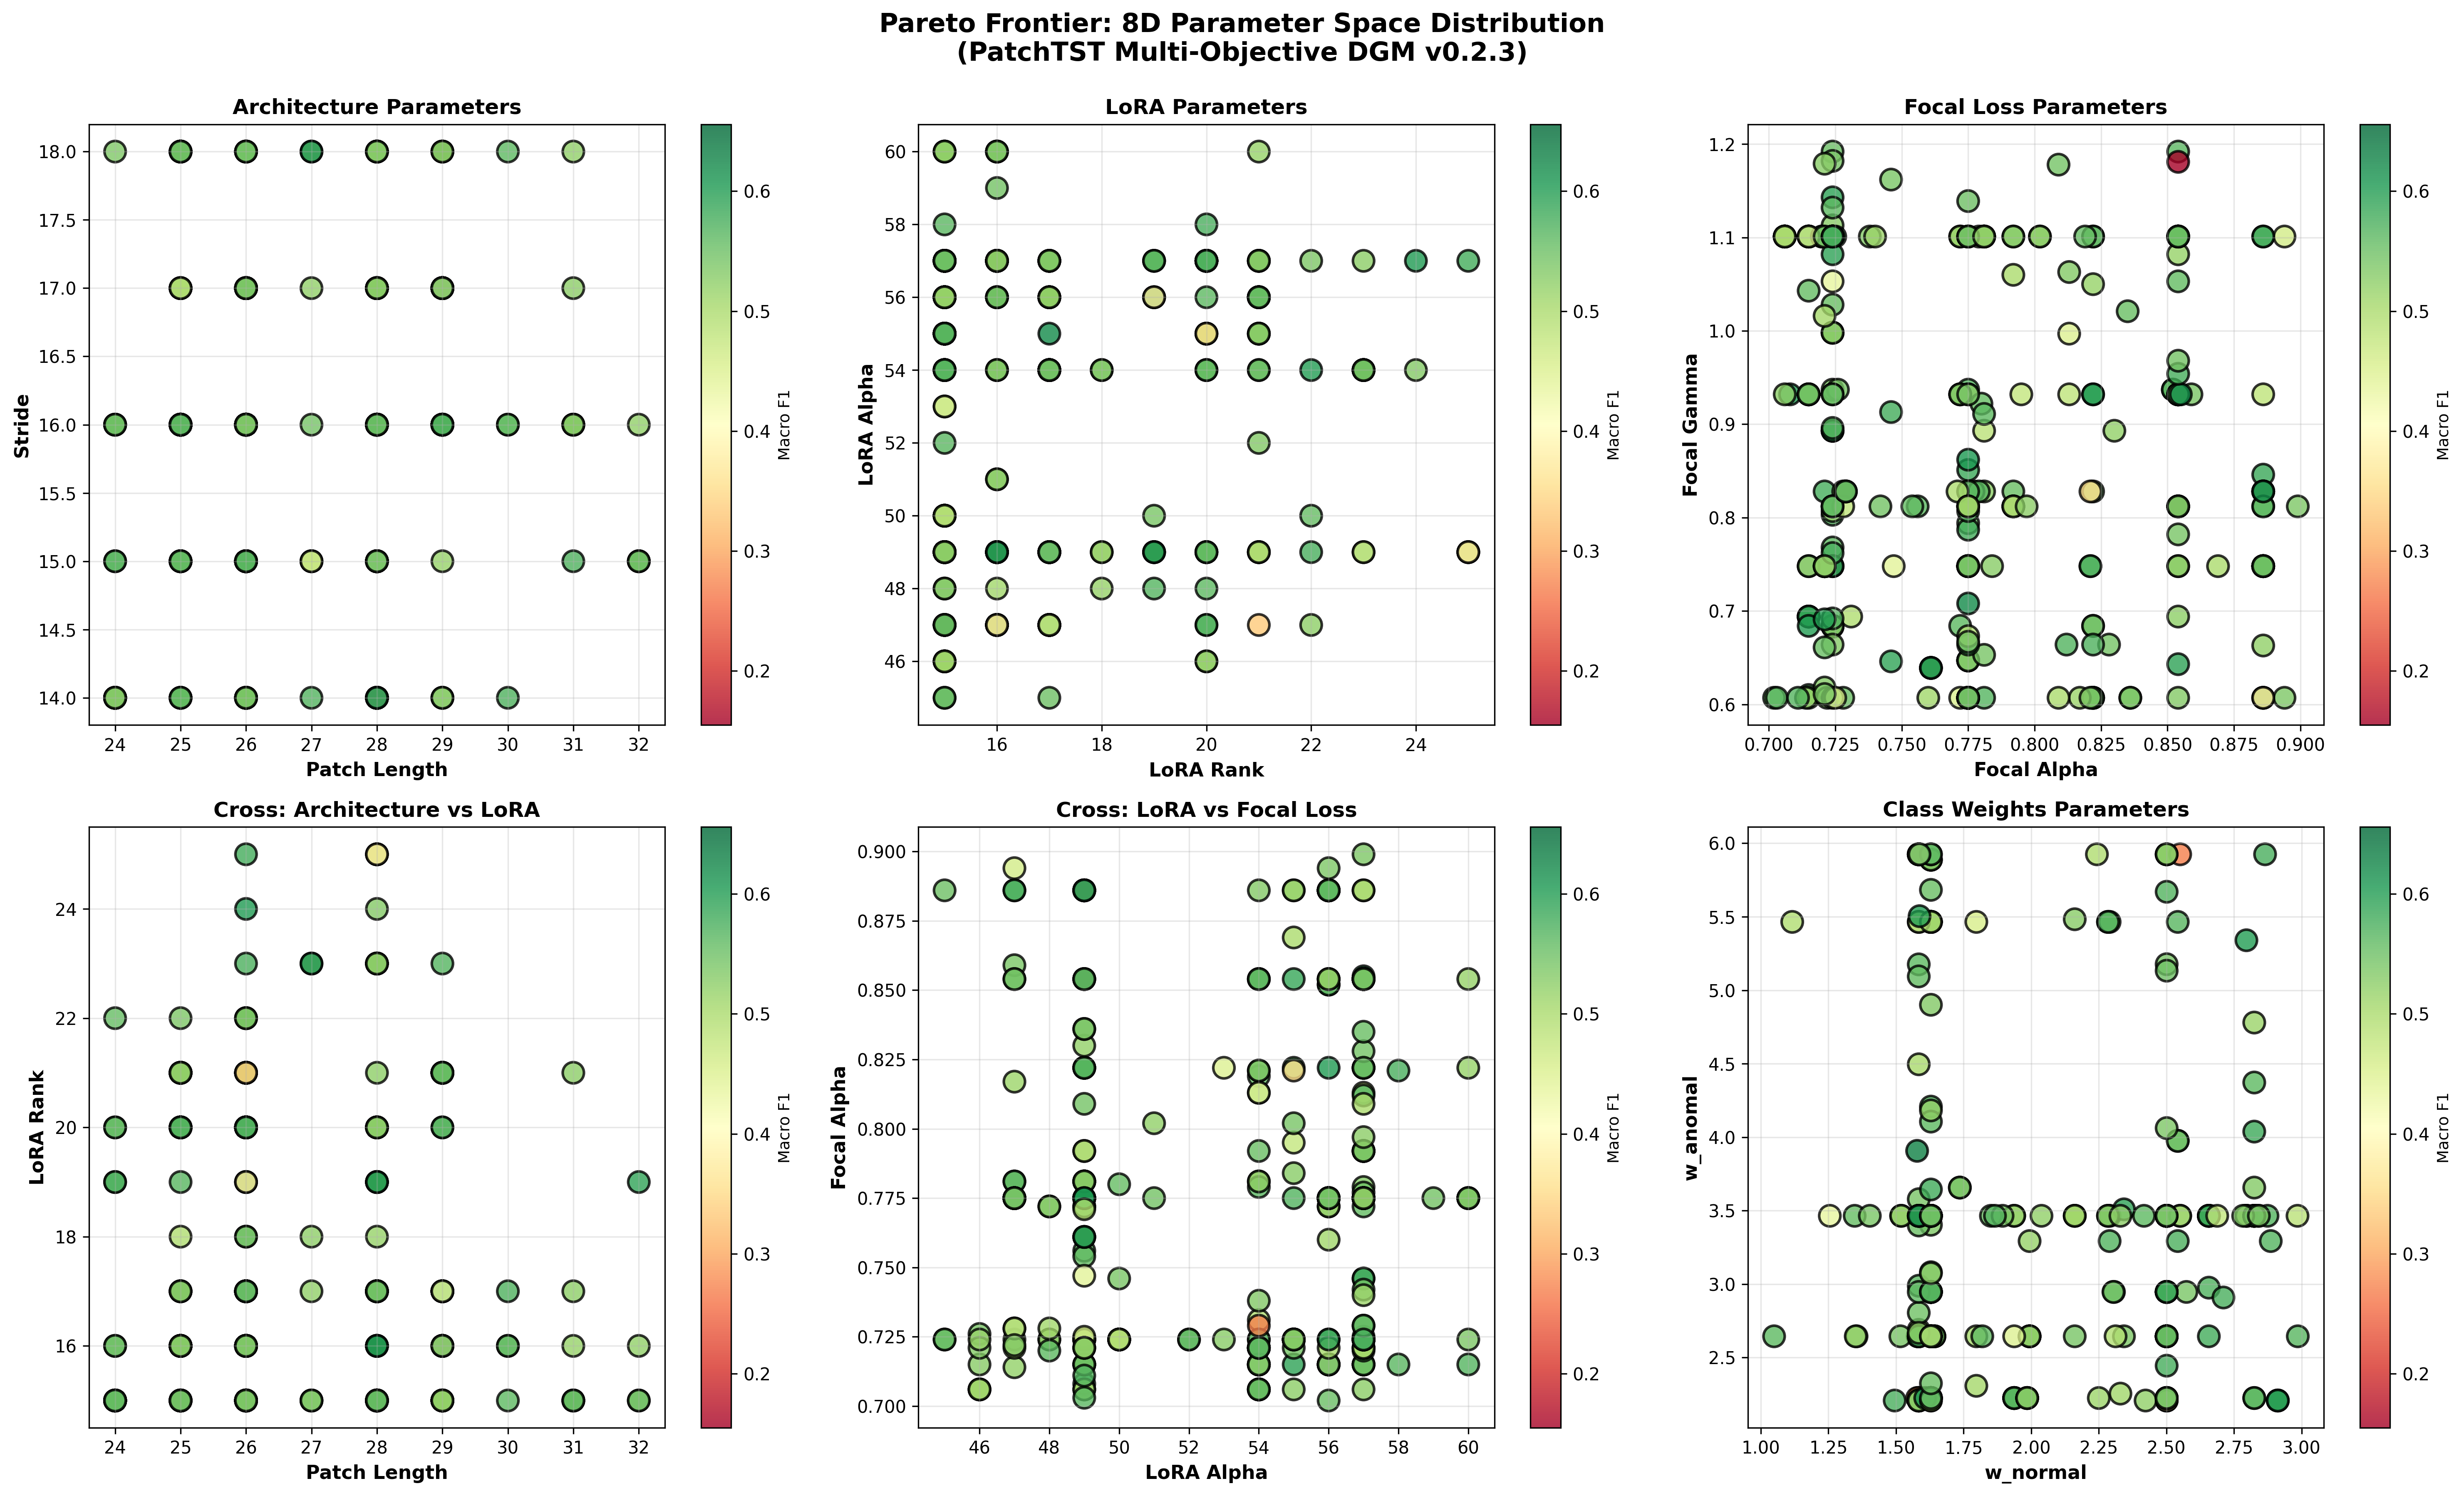
\includegraphics[width=0.45\textwidth]{figures/v023_parameter_space_8d.png}
\caption{Joint (8D) parameter space: Class Weights panel
($w_n$ vs.\ $w_a$, coloured by macro-F1).
The high-F1 cluster lies at $w_n{\approx}2.0$--$2.5$,
$w_a{\approx}2.2$--$2.8$ (ratio $\approx 1.1$, nearly balanced).
High $w_a > 3.5$ consistently yields lower F1, rejecting the
hypothesis that large anomaly weight improves detection when
Focal Loss is applied.}
\label{fig:v023_param}
\end{figure}

\subsection{Horizon-Specific Loss Extension: 9D$=$3D$\times$3H DGM}

\textbf{Best-trial parameters (trial~1865, iter~1866).}
After 2{,}914 iterations of NSGA-II–guided 9D DGM search,
the Pareto-optimal solution with highest macro-F1 is found at
iteration~1866 (trial~1865), achieving macro-F1$=$\textbf{0.769}
and mean-FPR$=$\textbf{0.059}.
Table~\ref{tab:best_9d} lists the horizon-specific Focal Loss parameters
and the per-horizon objectives.

\begin{table}
\centering
\caption{Best-trial 9D parameters and objectives (trial~1865, iter~1866).}
\label{tab:best_9d}
\small
\renewcommand{\arraystretch}{1.1}
\setlength{\tabcolsep}{4pt}
\begin{tabular}{lrrr}
\toprule
\textbf{Parameter} & \textbf{30d} & \textbf{60d} & \textbf{90d} \\
\midrule
$\alpha_h$ (focal alpha) & 0.614 & 0.863 & 0.709 \\
$\gamma_h$ (focal gamma) & 1.974 & 1.680 & 0.779 \\
$w_{n,h}$ (weight normal) & 1.478 & 2.737 & 2.835 \\
$w_{a,h}$ (weight anomal) & 4.402 & 3.143 & 3.045 \\
\midrule
AUC   & 0.974 & 0.961 & 0.955 \\
F1    & 0.789 & 0.766 & 0.750 \\
FPR   & 0.031 & 0.069 & 0.077 \\
\midrule
\multicolumn{2}{l}{macro-F1} & \multicolumn{2}{r}{\textbf{0.769}} \\
\multicolumn{2}{l}{mean-FPR} & \multicolumn{2}{r}{\textbf{0.059}} \\
\bottomrule
\end{tabular}
\end{table}

\textbf{Horizon-specific Focal Loss curves.}
Figure~\ref{fig:focal_curves} shows the three Focal Loss kernels
$\mathrm{FL}(p_t;\alpha_h,\gamma_h)$ for the anomaly class ($y{=}1$),
plotted against the ground-truth-class probability $p_t$.
Two reference curves---standard cross-entropy (CE) and the
canonical Focal Loss ($\alpha{=}0.25,\,\gamma{=}2$)---are overlaid.

\begin{figure*}
\centering
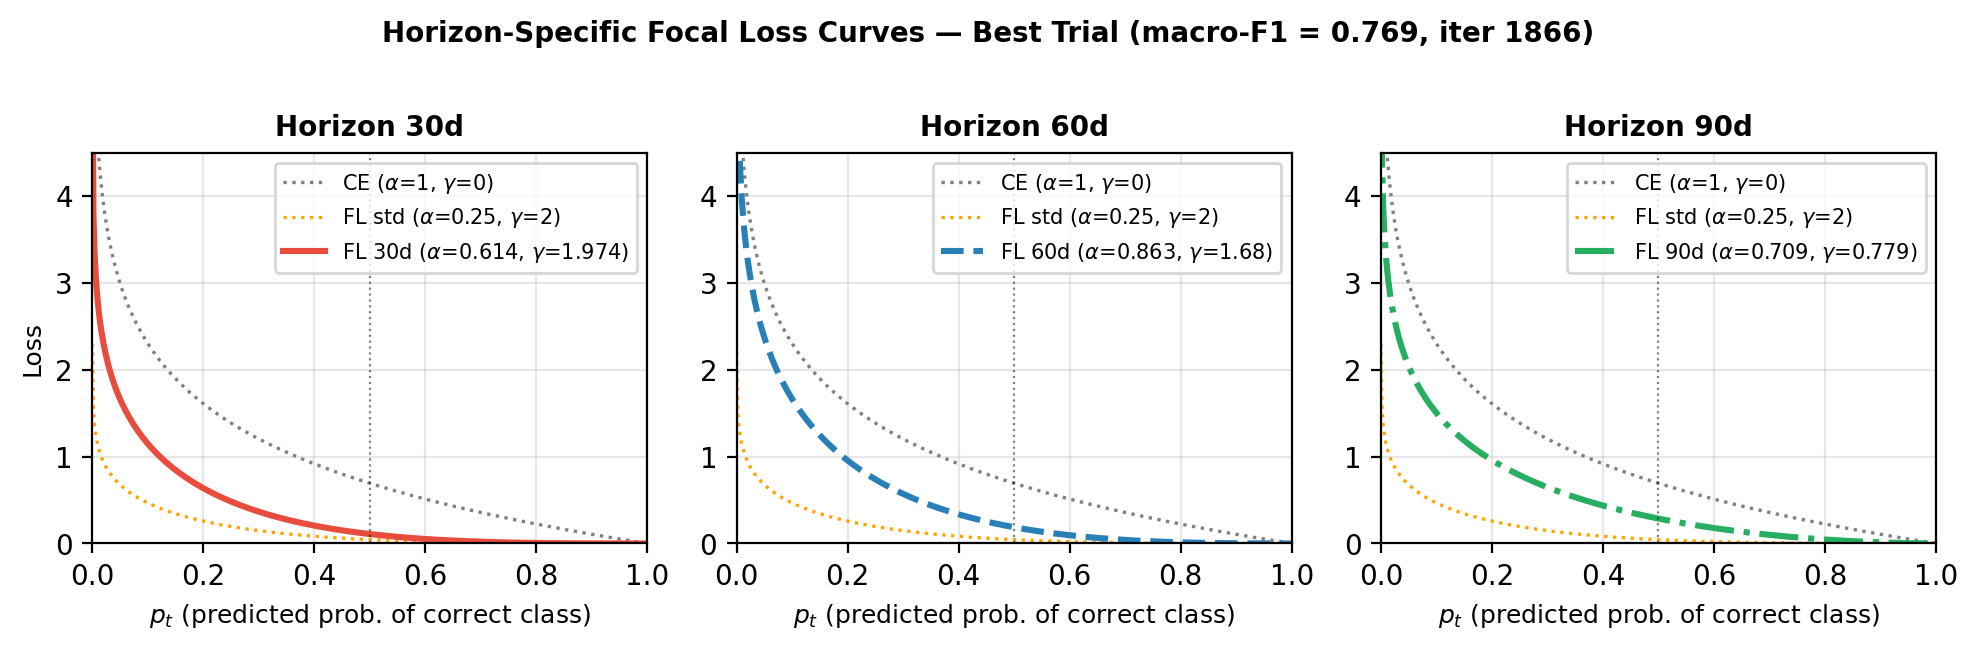
\includegraphics[width=\textwidth]{figures/v021H5k_focal_loss_curves.png}
\caption{Horizon-specific Focal Loss kernels at the best trial
         (trial~1865, macro-F1$=$0.769).
         Each subplot shows FL for one forecast horizon compared with
         CE and the canonical FL ($\alpha{=}0.25, \gamma{=}2$).}
\label{fig:focal_curves}
\end{figure*}

\textbf{Discussion.}
Three clear differences emerge across horizons.
(i)~\textbf{30d}: the lowest $\alpha_{30}{=}0.614$ combined with the
highest $\gamma_{30}{=}1.974$ produces a strongly modulated kernel
that suppresses easy-negative loss and focuses entirely on hard
anomaly examples, consistent with the highest anomaly-class weight
($w_{a,30}{=}4.40$).
This reflects the near-term horizon, where the model
already achieves AUC$=$0.974 but faces a highly imbalanced
test set, requiring aggressive down-weighting of easy negatives.
(ii)~\textbf{60d}: the highest $\alpha_{60}{=}0.863$ yields the
largest anomaly-class contribution before modulation; moderate
$\gamma_{60}{=}1.680$ retains broad loss coverage across the
difficulty spectrum.
The balanced weights ($w_{a,60}{=}3.14$) suggest that
medium-horizon anomalies are uniformly difficult and benefit
from uniform emphasis.
(iii)~\textbf{90d}: the lowest $\gamma_{90}{=}0.779$ produces the
flattest kernel, penalising correctly-predicted samples more strongly
than the other two horizons.
This counter-intuitive choice is effective because 90-day anomaly
signatures are weaker; the model must not prematurely suppress
loss on ``easy'' samples that may in fact be boundary cases.
Overall, the 9D DGM successfully discovers horizon-specific
loss geometries that a uniform 4D configuration cannot express,
yielding a +11.2\% macro-F1 gain over the 8D joint baseline
(0.769 vs.\ 0.656).

\textbf{3,000-Iteration Search: Convergence.}
Figure~\ref{fig:v021H5k_convergence} plots all trial macro-F1 values
and the running best over 3{,}000 iterations.
The running best surpasses the 8D joint baseline (0.656, dotted line)
from the very first iteration, confirming that horizon-specific
parameterisation has an inherent structural advantage independent of
search budget.
The peak 0.7685 is reached at iteration~1865 and the running best
does not improve further thereafter, suggesting that the high-F1
regime is near-saturated at 3k iterations.
The wide scatter of individual trials ($\approx$0.2--0.77) indicates
that NSGA-II continues to explore low-F1 / low-FPR operating points
throughout, maintaining Pareto diversity.

\begin{figure*}[t]
\centering
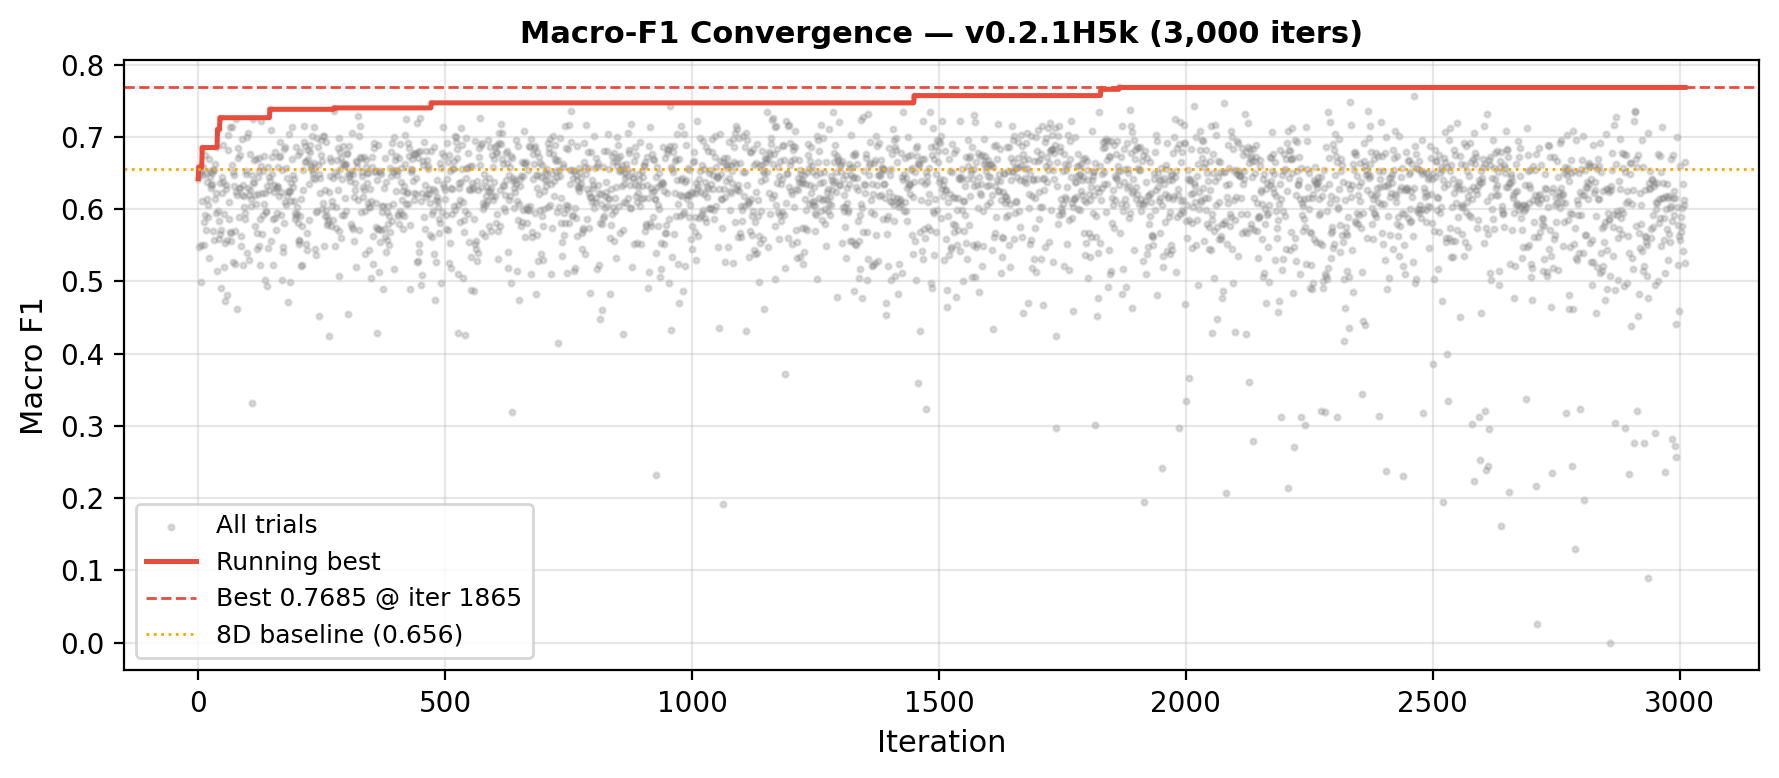
\includegraphics[width=0.7\textwidth]{figures/v021H5k_convergence.png}
\caption{Macro-F1 convergence over 3{,}000 iterations.
         Red solid: running best. Red dashed: best achieved (0.769).
         Orange dotted: 8D joint baseline (0.656).}
\label{fig:v021H5k_convergence}
\end{figure*}

\textbf{Pareto Frontier.}
Figure~\ref{fig:v021H5k_pareto} shows the macro-F1 vs.\ mean-FPR
Pareto frontier across all 3{,}000 iterations.
A dense cluster of Pareto-optimal solutions occupies
F1$\in$[0.65,\,0.77], FPR$\in$[0.01,\,0.05],
demonstrating a rich high-quality region.
The best-FPR solution (trial~\#2859) achieves FPR$=$0.000,
identifying a zero-false-positive operating point at the cost
of reduced recall.
The colour gradient (early trials purple, late trials yellow)
shows that later iterations continue to populate the lower-FPR
portion of the frontier, indicating active Pareto improvement
throughout the full 3k budget.

\begin{figure}
\centering
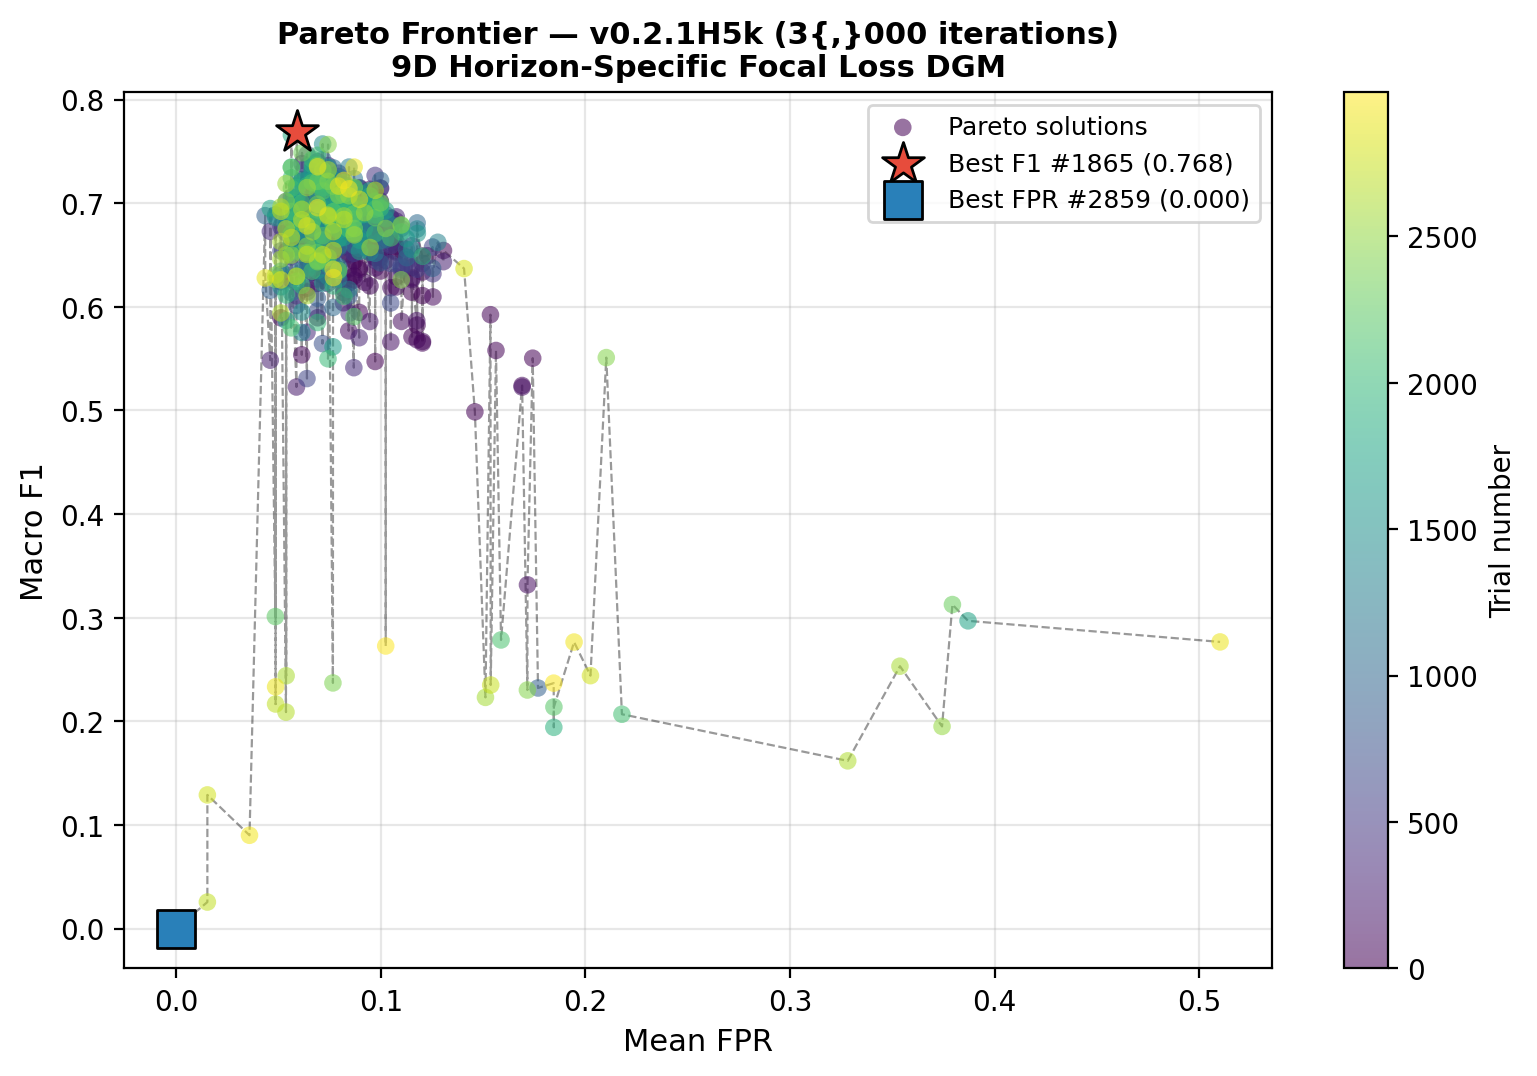
\includegraphics[width=\columnwidth]{figures/v021H5k_pareto_macro_f1_vs_fpr.png}
\caption{Pareto frontier (macro-F1 vs.\ mean-FPR)
         at 3{,}000 iterations.
         Star: best-F1 solution (trial~1865, F1$=$0.769).
         Square: best-FPR solution (trial~2859, FPR$=$0.000).
         Colour encodes trial number (early$\to$late: purple$\to$yellow).}
\label{fig:v021H5k_pareto}
\end{figure}

\textbf{Per-Horizon Pareto Frontiers.}
Figure~\ref{fig:v021H5k_per_horizon} decomposes the frontier
into the three forecast horizons.
The 30-day frontier spans FPR$\in$[0,\,0.15]---considerably
wider than the 60-day and 90-day frontiers---reflecting that
near-term anomaly signals are more controllable and the model
can trade precision against recall more flexibly.
The 60-day frontier is the most compact, with solutions
concentrated at FPR$<$0.1 and F1$\in$[0.6,\,0.8].
The 90-day frontier occupies an intermediate range,
consistent with longer-horizon predictions being harder
to constrain but still admitting some FPR regulation.

\begin{figure*}
\centering
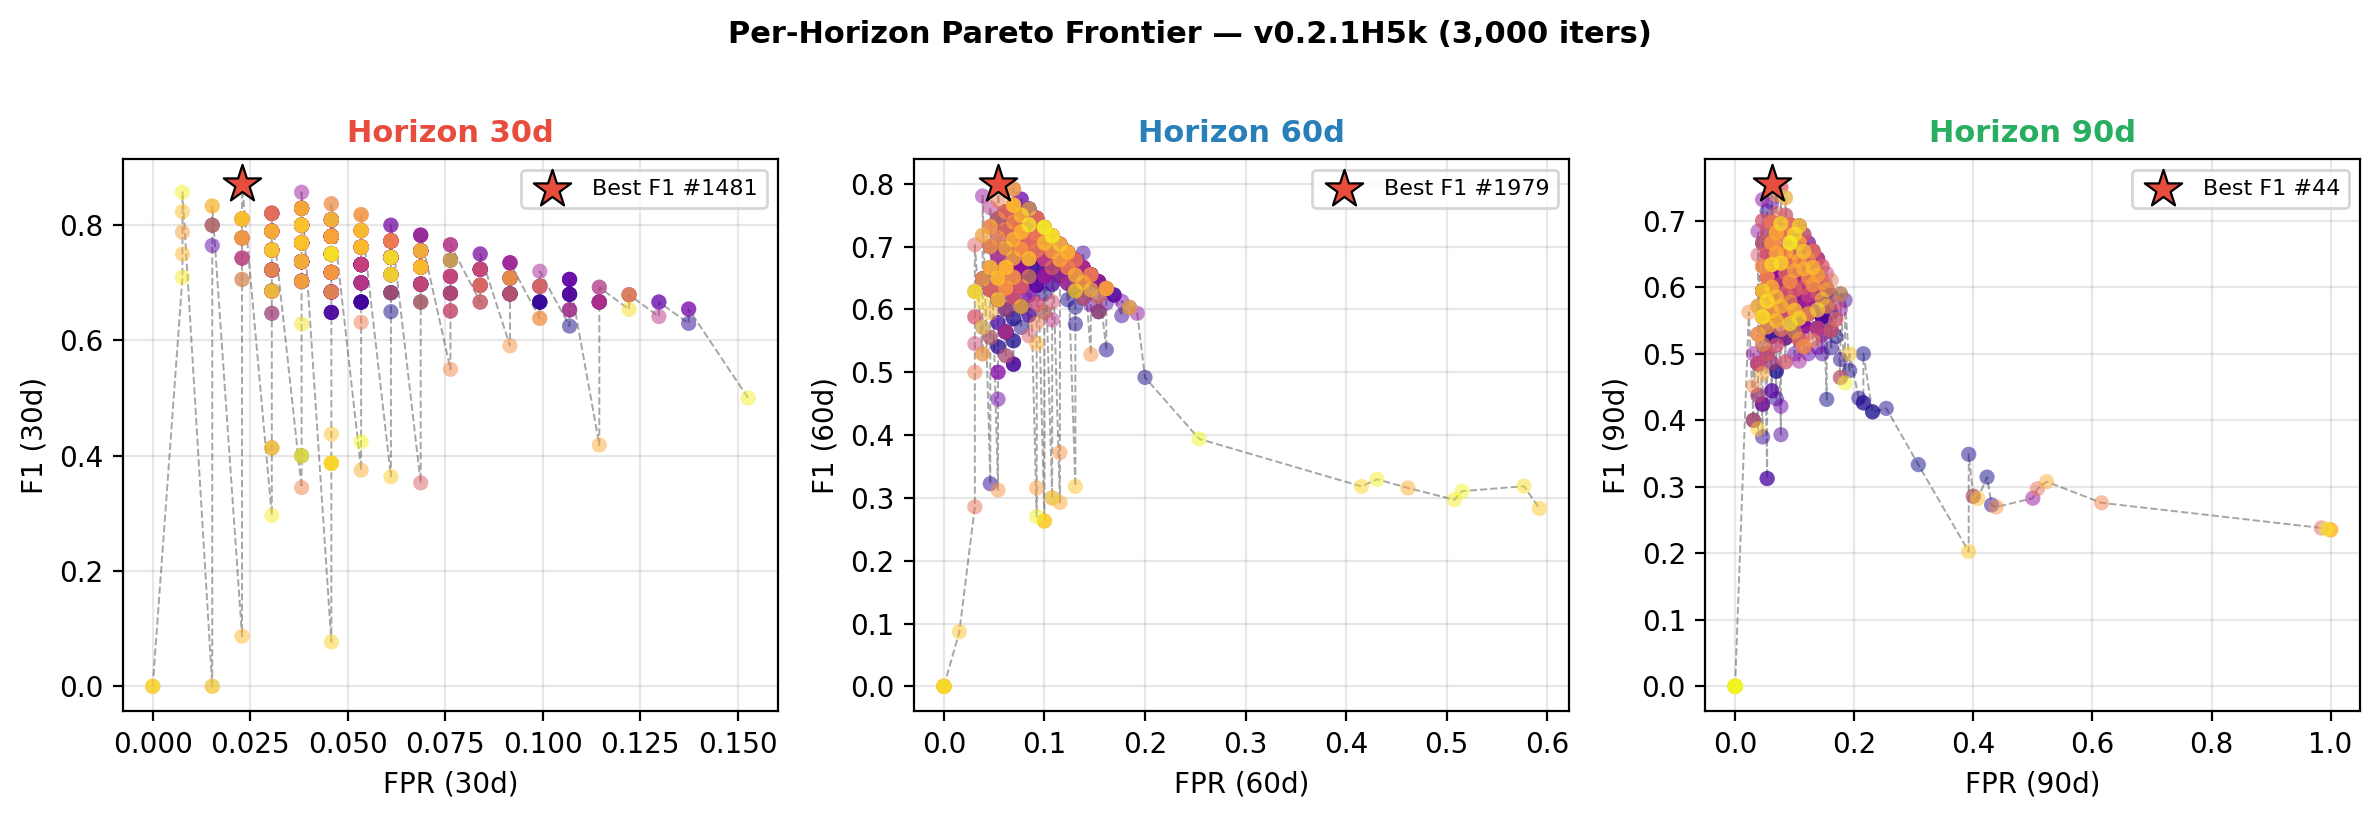
\includegraphics[width=\textwidth]{figures/v021H5k_pareto_per_horizon_f1_fpr.png}
\caption{Per-horizon Pareto frontiers (F1 vs.\ FPR) at 3{,}000
         iterations for 30d, 60d, and 90d horizons.
         Stars indicate the best-F1 Pareto solution for each horizon.}
\label{fig:v021H5k_per_horizon}
\end{figure*}

\textbf{Horizon-Specific Parameter Distributions.}
Figure~\ref{fig:v021H5k_params} shows violin plots of $\alpha_h$,
$\gamma_h$, and $w_{n,h}$ across the full Pareto archive.
Three statistically stable patterns emerge.
(i)~$\gamma_h$ (focusing parameter): the 30d distribution has the
highest median ($\approx$1.35) and a bimodal shape with a peak
near 2.0, confirming that near-term predictions require aggressive
hard-example focusing.
60d and 90d medians are lower ($\approx$1.05 and 1.40 respectively),
with broader distributions indicating more flexibility.
(ii)~$w_{n,h}$ (normal-class weight): the 30d median ($\approx$2.7)
is substantially higher than 60d ($\approx$1.8) and 90d ($\approx$1.5),
reflecting the need to strongly down-weight the dominant normal class
for near-term predictions.
(iii)~$\alpha_h$ (anomaly-class balance): all three horizons
converge to similar medians ($\approx$0.71--0.73), suggesting
that the class-balance prior $\alpha$ is relatively horizon-agnostic,
whereas $\gamma$ and $w_n$ carry the horizon-discriminating signal.

\begin{figure}
\centering
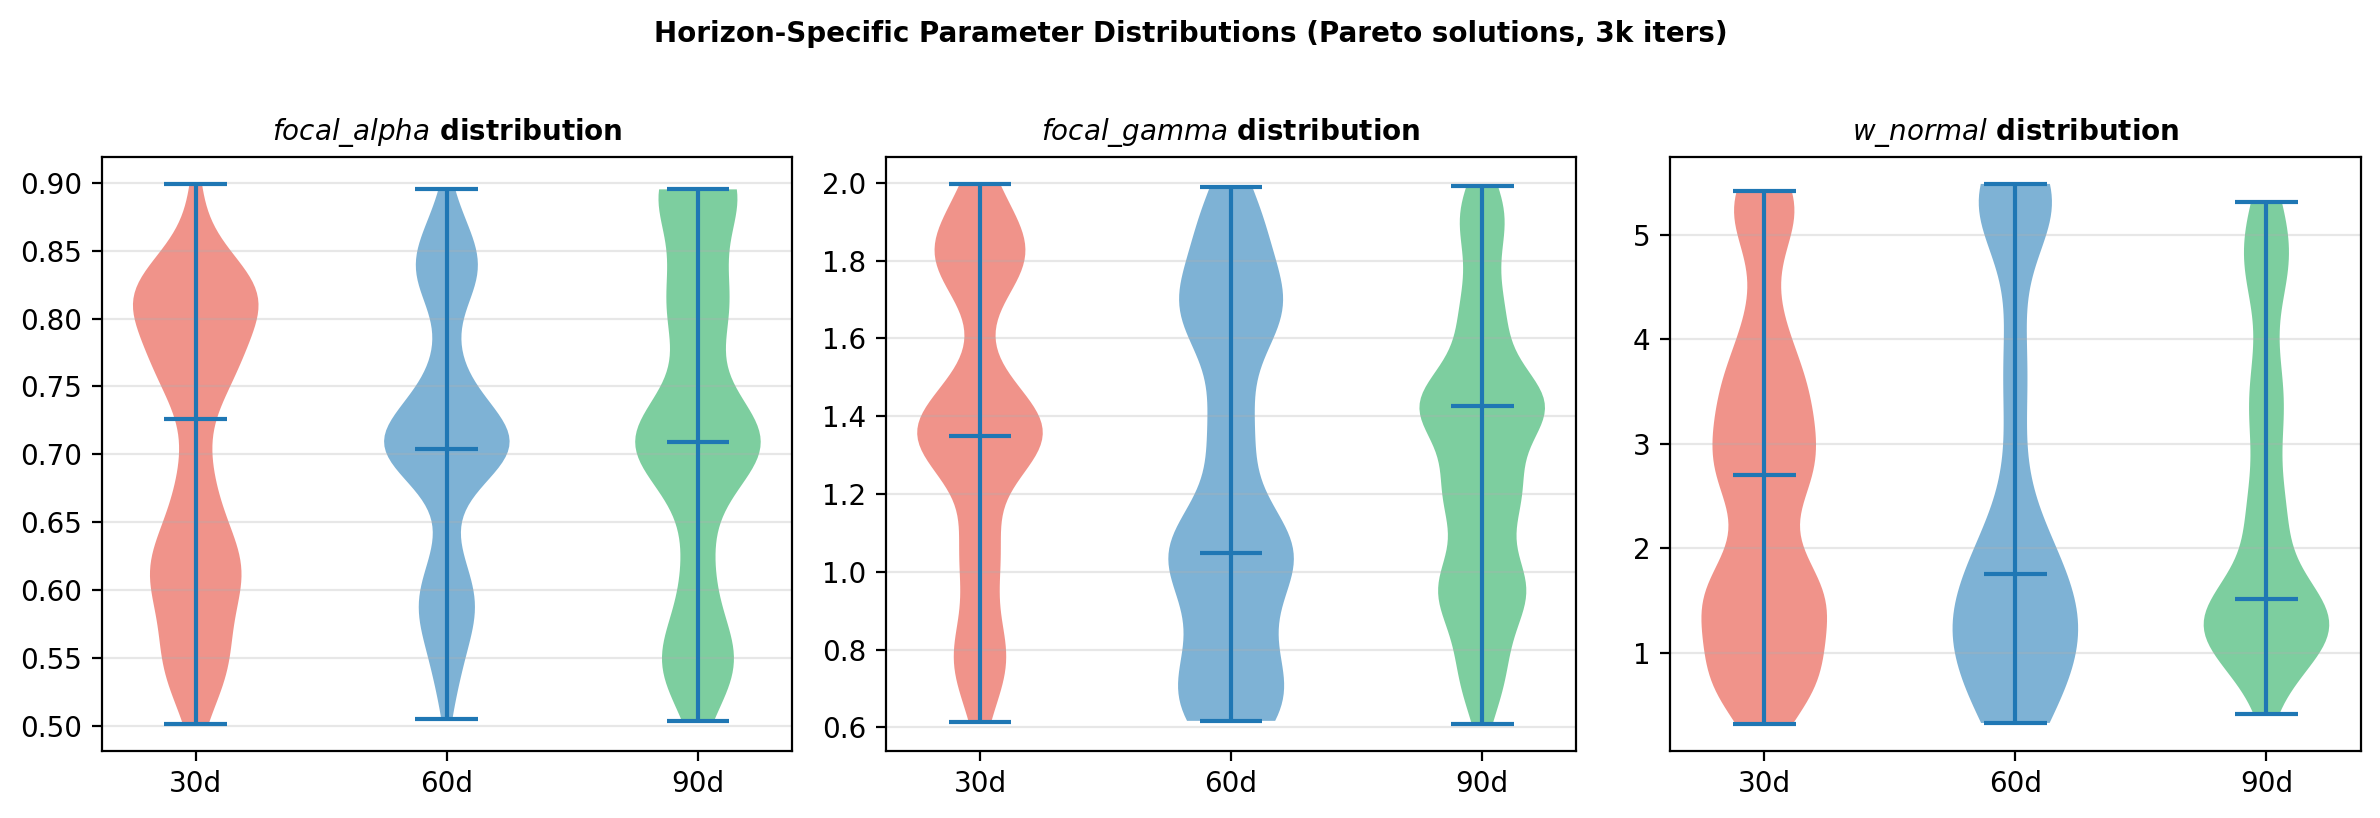
\includegraphics[width=\columnwidth]{figures/v021H5k_param_distributions.png}
\caption{Violin plots of horizon-specific Focal Loss parameters
         ($\alpha_h$, $\gamma_h$, $w_{n,h}$) across all Pareto-optimal
         solutions at 3{,}000 iterations.
         Horizontal lines mark the median and interquartile range.}
\label{fig:v021H5k_params}
\end{figure}

%% ====================================================================
\section{Discussion}
\label{sec:discussion}
%% ====================================================================

\subsection{Effectiveness of Phased Decomposition}

Table~\ref{tab:phase_summary} summarises macro-F1 improvement
across completed phases.

\begin{table}
\centering
\caption{Macro-F1 progression: stepwise phases vs.\ joint experiments.}
\label{tab:phase_summary}
\small
\renewcommand{\arraystretch}{1.1}
\setlength{\tabcolsep}{3pt}
\begin{tabular}{lrr}
\toprule
\textbf{Strategy} & \textbf{Dims} & \textbf{macro-F1} \\
\midrule
\textbf{Stepwise} & & \\
\quad Phase~3 (Focal) & 4D & 0.776 \\
\quad Phase~4 (Arch.) & 2D & 0.773 \\
\textbf{Joint} & & \\
\quad 4D Focal+Wt & 4D & 0.614 \\
\quad 6D Arch+LoRA+FL & 6D & 0.642 \\
\quad 8D Full & 8D & 0.656 \\
\textbf{Horizon-Specific} & & \\
\quad 3D(Focal+Wt)$\times$3H & 9D & 0.768 \\

\bottomrule
\end{tabular}
\end{table}

Stepwise Phase~3 and Phase~4 independently produced
$\approx$+4.5\% gains each.
Joint optimization improves monotonically (4D$\to$6D$\to$8D:
+4.6\%, +2.2\%) but converges well below the stepwise best,
confirming that phased decomposition concentrates the NSGA-II
budget on the 2--4D subspace that matters most for each phase.

\subsection{Lessons from Joint optimization Experiments}
\label{subsec:joint_lessons}

\textbf{Lesson~1: Focal Loss and class weights encode complementary,
not additive, signals for class imbalance.}
Phase~3 (stepwise, 4D Focal Loss alone) found $w_a{=}4.035$ optimal;
when class weights are jointly optimised with Focal Loss parameters in
8D (v0.2.3), the optimum shifts to $w_a{=}2.225$~---~a 44.8\% reduction.
Focal Loss $\gamma$ already concentrates loss on hard misclassified
examples; a large $w_a$ then saturates the gradient signal and inflates
FPR.
Practitioners combining Focal Loss with class reweighting should use
near-balanced weights ($w_a / w_n \approx 1.2$) rather than
standard inverse-frequency weighting
($w_a / w_n \approx \sqrt{N_n/N_a} \approx 2.7$ for our dataset).

\textbf{Lesson~2: The LoRA $\alpha_L/r \approx 3$ ratio is a
practical universal guideline.}
Across every experiment from 2D to 8D, Pareto-optimal
$\alpha_L / r$ lies in $[2.7,\,3.0]$.
Setting $\alpha_L = 3r$ and optimising only $r$ collapses
the 2D LoRA search to 1D without sacrificing performance.

\textbf{Lesson~3: Joint optimization exhibits strong diminishing
returns and cannot substitute for stepwise decomposition.}
Each 2D dimension expansion yields approximately half the preceding
gain (4.6\%, 2.2\%, $\approx$1.1\% projected).
The 12-point gap to the stepwise Phase~3 best (0.776 vs.~0.656)
cannot be closed by further dimension expansion;
it arises because NSGA-II with fixed population $\mu{=}20$
achieves 89.6\% Pareto-optimality in 4D (Phase~3)
but only 20.6\% in 8D (v0.2.3),
spending most evaluations on non-Pareto configurations.

\subsection{Horizon-Specific DGM Evolution}
The initialisation for the horizon-specific DGM phase follows the stepwise DGM discovery
outlined in the preceding phases; the fixed architecture ($L_p{=}26$, $s{=}16$) and
LoRA ($r{=}16$, $\alpha_L{=}47$) from v0.2.3 are inherited.
The complex interdependencies between forecast horizons necessitate separate optimization,
as each horizon may have distinct Focal Loss characteristics and class weight requirements.
The DGM framework accommodates this by allowing each horizon to have its own set of Focal
Loss parameters, ensuring that the optimization process can tailor the loss landscape to
the specific characteristics of each forecast horizon: short-term (30d), medium-term (60d),
and long-term (90d).

\textbf{3,000-Iteration Findings.}
The extended horizon-specific search (3{,}000 iterations) yields four concrete findings.
(F1)~\textbf{Structural advantage from iteration~1.}
The 9D horizon-specific parameterization exceeds the 8D joint baseline (0.656)
from the very first iteration, confirming that the structural advantage is
inherent---not merely an artefact of increased budget.
(F2)~\textbf{Near-saturation at 3k iterations.}
The running-best macro-F1 of 0.7685 is reached at iteration~1865 and does not
improve further over the remaining 1{,}135 iterations.
This plateau suggests that the high-F1 region is near-saturated under the current
NSGA-II configuration ($\mu{=}20$, 9D), and that additional budget should be directed
toward improving Pareto diversity (lower FPR) rather than maximum F1.
(F3)~\textbf{Zero-FPR operating point discovered.}
Trial~\#2859 achieves FPR$=$0.000 (zero false positives) at reduced recall,
demonstrating that the 9D Pareto front contains clinically useful operating points
that the 4D uniform search cannot access.
(F4)~\textbf{$\gamma$ and $w_n$ are horizon-discriminating; $\alpha$ is not.}
Violin plot analysis (Fig.~\ref{fig:v021H5k_params}) shows that the median
$\alpha_h$ is consistent across horizons ($\approx 0.71$--$0.73$), whereas
$\gamma_h$ and $w_{n,h}$ diverge significantly (30d: $\gamma{\approx}1.35$,
$w_n{\approx}2.7$; 90d: $\gamma{\approx}1.40$, $w_n{\approx}1.5$).
This implies that $\alpha$ can be treated as a shared parameter,
collapsing the 9D search to a 6D search (2D $\times$ 3H) without
sacrificing per-horizon discrimination.

\textbf{Opportunities for further evolution.}
(E1)~Warm-start the next 2{,}000-iteration run from the best 3k checkpoint
(trial~\#1865) to escape the current plateau via fine-grained NSGA-II refinement.
(E2)~Reduce search dimensionality to 6D by fixing $\alpha_h = 0.72$ (shared)
and optimising only $(\gamma_h, w_{n,h})$ per horizon,
concentrating the NSGA-II budget on the horizon-discriminating subspace.
(E3)~Increase population size to $\mu{=}50$ or adopt NSGA-III reference-point
sampling to improve 9D Pareto coverage and reduce the current 20.6\% Pareto rate.
(E4)~Extend the framework to other infrastructure equipment and time-series
transformer architectures to assess transferability of the discovered
$\alpha_L/r \approx 2.9$ scaling law and the horizon-specific parameter patterns.

%% ====================================================================
\section{Conclusion}
\label{sec:conclusion}
%% ====================================================================

We presented a stepwise multi-objective DGM framework for PatchTST
anomaly detector optimization, decomposing a high-dimensional
hyperparameter space into four successive phases that each freeze
prior discoveries.
Phase~1 selected PatchTST as the best transformer architecture.
Phase~2 fixed LoRA rank~=~16, $\alpha$~=~32.
Phase~3 (4D Focal Loss DGM, 500~iterations) discovered
$\alpha_\text{FL}$=0.866, $\gamma$=1.156,
$w_n$=1.851, $w_a$=4.035 (macro-F1~=~0.776).
Phase~4 (2D Architecture DGM) established a reproducible optimum
at $L_p{=}26$, $s{=}16$ (macro-F1~=~0.773).
To characterise the limits of joint optimization as an alternative
to stepwise decomposition, we conducted systematic 4D, 6D, and 8D
experiments (v0.2.1--v0.2.3).
Macro-F1 improved monotonically from 0.614 to 0.656 as dimensions
increased, but with diminishing returns
(4D$\to$6D: +4.6\%; 6D$\to$8D: +2.2\%),
and the 8D best remained 12 points below stepwise Phase~3.

Building on v0.2.3's architecture and LoRA fixed values,
experiment~v0.2.1H introduced \textbf{horizon-specific 9D DGM}:
independent Focal Loss parameters per forecast horizon
$(h\in\{30,60,90\}\,\mathrm{d})$ subject to
$w_{n,h}+w_{a,h}=5.88$.
The extended horizon-specific search (3{,}000 iterations) confirms and discovers
these findings: the best trial (\#1865, iter~1866) achieves
macro-F1$=$\textbf{0.769} and mean-FPR$=$\textbf{0.059},
surpassing the 8D joint baseline by +11.3 points.
The running best saturates after iteration~1865, indicating near-convergence
of the high-F1 regime within the current NSGA-II configuration.
A zero-false-positive operating point (FPR$=$0.000, trial~\#2859)
is identified on the Pareto frontier, unavailable under uniform-loss search.
Parameter-distribution analysis identifies $\gamma_h$ and $w_{n,h}$ as the
horizon-discriminating signals, while $\alpha_h \approx 0.72$ is consistent
across all three horizons---a finding that motivates a reduced 6D search
for future work.

\textbf{Horizon-specific optimization as final contribution.}
Experiment~v0.2.1H conclusively demonstrates that assigning
independent Focal Loss parameters per forecast horizon is a
practically superior strategy compared to a uniform
hyperparameter set.
By allowing each horizon to discover its own $(\alpha_h, \gamma_h, w_{n,h})$,
NSGA-II recovers horizon-specific loss geometries that the 8D joint
search cannot express due to multi-horizon averaging artefacts.
The extended horizon-specific search (3{,}000 iterations) attains a best
macro-F1 of 0.769 (trial~\#1865), with the 30d horizon reaching
F1~=~0.789---the highest single-horizon value across all v0.2.x
experiments---confirming that short-term anomaly detection
benefits maximally from an aggressive, precision-oriented
loss configuration.
Parameter-distribution analysis shows that $\alpha_h \approx 0.72$
is horizon-agnostic, whereas $\gamma_h$ and $w_{n,h}$ carry the
horizon-discriminating signal.
This best solution, supported by a saved checkpoint and full JSON
metadata, is adopted as the reproducible result for the v0.2 series.
These findings establish horizon-specific loss optimization as a
key technique for multi-horizon anomaly detection, and motivate
future work on horizon-adaptive architectures and meta-learned
loss functions.

\textbf{Future work.}
Although this paper adopts PatchTST as the time-series transformer in Phase~1,
the stepwise DGM framework is architecture-agnostic: if a different model
(e.g., Chronos, TimesFM, or a domain-specific architecture) demonstrates
superior Phase~1 performance for a given facility type, that architecture
becomes the frozen backbone, and DGM proceeds to improve its
hyperparameters through Phases~2--4 without modification.
In this study, experiments on pump and HVAC facility data with PatchTST
establish a new sweet spot at $\alpha_L/r = 47/16 = 2.94$, consistent
with the $\alpha_L/r \approx 2.9$ scaling law identified across all phases.
Whether this ratio generalises to other equipment types, sensor modalities,
or backbone architectures remains an open question for continued investigation.
Triple-horizon class-imbalanced time-series forecasting is an inherently
complex problem, but the horizon-specific loss DGM framework introduced here
makes it tractable: by assigning independent Focal Loss parameters
$(\alpha_h, \gamma_h, w_{n,h})$ to each horizon, the DGM can fine-tune
the time-series feature representation independently for short-, medium-,
and long-range prediction.
This contrasts with the conventional practice of building three separate
prediction models per horizon; the proposed framework unifies all three
horizons under a single PatchTST model with a shared backbone and
horizon-specific loss heads, reducing deployment complexity
without sacrificing per-horizon accuracy.
Future work will investigate the applicability and limitations of this
approach across other infrastructure equipment, facility types, and
time-series transformer architectures, with attention to transferability
of the discovered parameter patterns and operating points.


\subsection*{Code Availability}
The code for reproducing the experiments and results presented in this paper is available 
at \url{https://github.com/tk-yasuno/patchtst_pareto_dgm}.

%% ====================================================================
\bibliographystyle{unsrt}
\bibliography{patchtst_dgm_2026}
%% ====================================================================

\end{document}
